\chapter{Effect of geometrical parameters and inertia on the apparent permeability tensor in fibrous porous media}
\label{ch:4}


\chapquote{It is far better to foresee even without certainty than not to foresee at all.}{The Foundations of Science}{Henri Poincare}

%%%%%%%%%%%%%%%%%%%%%%%%%%
\section{Introduction}
%%%%%%%%%%%%%%%%%%%%%%%%%%

Include this paper \citet{penha2011computing} and this one \citet{firdaouss1997nonlinear}

The flow through porous media is a problem of importance for several natural and technological applications. Since Darcy's original
formulation \cite{darcy}, which relates the flow rate through a porous bed to the pressure drop across the bed's sides, many
corrections have been made to account, for example, for viscous effects \cite{brinkman} or for the consequences of inertia \cite{forchheimer}.  
All of the cited works are of empirical nature, but homogenisation has been able to recover all of these
formulations rigorously starting from the Navier-Stokes equations \cite{whitaker2013method}. This latter approach is sometimes defined 
VANS, for Volume-Averaged Navier-Stokes.

The theory requires the knowledge of a number of terms, most notably, in the case of an isotropic porous bed, a permeability
coefficient and a Forchheimer coefficient. Initial efforts in defining these terms were based on a combination of physical
reasoning and measurements, leading to  expressions known as the Kozeny-Carman \cite{kozeny, carman} and the Ergun \cite{ergun}
correlations. The first provides the permeability for the laminar flow of a single-phase fluid through a packed bed of sand grains, 
as function of the porosity and the diameter of the grains, while the second extends Darcy's law to let the pressure drop depend on 
two terms, one proportional to the velocity and the second to its square, thus accounting for inertia. These approaches do not consider 
microstructural or geometrical features of the porous bed, which can render the permeability a tensorial quantity, and are often restricted 
to simple unidirectional flows.  In the present work we are concerned with a transversely isotropic material composed by parallel
fibers of circular cross-section, with one axis of symmetry, $(O,x_3)$; in such materials the permeability is a diagonal tensor
with the component in the direction parallel to the fibers greater than those along the transverse axes. For such an arrangement
we will investigate the effects of both the direction of the forcing pressure gradient and inertia. When the latter effect is present,
embodied by a Reynolds number $Re_d$, based on mean velocity through the medium and fibers' diameter, exceeding an order one threshold, 
the permeability is no more simply defined upon geometrical properties. This new permeability, which arises from a well-defined closure
problem, is then called \emph{apparent permeability}.

The influence of the geometry of the solid inclusions has been addressed previously by \citet{yazdchi2011} for arrays of cylinders 
in both square and hexagonal (or staggered) patterns, with the cylinders' section which can vary in shape. The results, in the 
two-dimensional and low Reynolds number limits, demonstrate the dependence of the  permeability component along the flow direction to both 
the porosity and the direction of the macroscopic pressure gradient. The direction of the pressure gradient is found to have a weak effect 
for beds of medium-high porosity ($\varepsilon>0.7$) and a stronger dependence appears upon the geometry of the solid inclusions. 
%An interesting observation made by \citet{yazdchi2011} concerns the relation between the angle of the staggered cell arrangement 
%and the permeability, particularly for medium-high porosities.

%In \citet{lasseux} the authors study the problem of the inertia correction on the Darcy law (Forchheimer tensor), and its relation 
%with the Reynolds number and the orientation of the mean pressure gredient.
The influence of the Reynolds number on the permeability and on the Forchheimer correction has been presented in a number of papers.
One of the contributions most relevant here is due to \citet{edwards1990}. These authors show that, for arrays of fibers, the apparent permeability decreases with the increase of the Reynolds number, and the rate of this decrease depends on the geometry of the array;
also, the Reynolds number is found to have a stronger influence on the apparent permeability when the medium is highly porous.
The results of the work by \citet{edwards1990} agree with those by \citet{zampogna} and with our own work (as shown later), all for
the case of cylindrical fibers, although some issues remain on the persistence of steady solutions in the simulations by \citet{edwards1990} 
in cases for which a limit cycle should have set in. A fully three-dimensional porous medium, more complex than those discussed so far, 
has been considered by \citet{soulaine2014}, confirming the decreasing trend of the apparent permeability with the Reynolds number. 

Another contribution which deserves mention is that by \citet{lasseux}; they have computed the permeability tensor 
for various Reynolds numbers, in a two-dimensional geometry with cylinders of square cross-section.
Forcing the flow along the main symmetric directions of the fiber, \citet{lasseux} have identified different regimes:
\begin{itemize}
	\item a creeping flow regime for $ 0 < Re_d < 10^{-3}$, without Forchheimer terms;
	\item a weak inertia regime for $10^{-3} < Re_d < 1$, with the Forchheimer correction quadratic in $Re_d$; 
	\item a strong inertia regime for $1 < Re_d < 10$, where the Forchheimer correction is linear with the Reynolds number; 
	\item a turbulent regime, for  $Re_d > 10 $, with the Forchheimer correction again quadratic with the Reynolds number.
\end{itemize}  
The boundaries between the different regimes are specific to the geometrical arrangements and to the porosities being considered; 
a step forward in rendering (some of) these boundaries rigorous and independent of the arrangement of the pores, through the definition 
of a Reynolds number which accounts for a ''topological" coefficient, has been recently made by \citet{pauthenet}. 
For the purposes of the present paper, we must retain that \citet{lasseux} have parametrized the Forchheimer correction with the Reynolds 
number, and have found that the inertial correction is orders of magnitude smaller than the Darcy's term, at least before the turbulent 
regime sets in. Moreover, \citet{lasseux} have studied how a Forchheimer tensor, $\mathbf{F}$, depends upon the direction of the
macroscopic forcing term with respect to the orientation of the square cross-section of the fibers, for  $Re_d$ up to 30.
It is concluded that a deviation angle, $\gamma$, exists between the direction of the pressure gradient and that of the mean flow,
because of the fibers' geometry. Finally, the inertial correction is strongly influenced by the orientation
of the driving pressure gradient, and the tensor $\mathbf{F}$ is not symmetric (in fact the off-diagonal components 
are found to be inversely proportional to the diagonal terms, and symmetric with respect to rotations about the diagonal axis of 
the square, i.e. the direction at $45^\circ$ in the $x_1 - x_2$ plane).

The effect of variations in the forcing angle, with restrictions to angles in the $x_1 - x_2$ plane, is also examined by 
\citet{soulaine2014} with conclusions in qualitative agreement with those of  both the contribution just cited and our results  
described further below. In all cases, the off-diagonal components of the apparent permeability tensor are small and the diagonal 
components display but a small variation upon rotation of the driving pressure gradient.


As already anticipated, this work investigates how thedirection of the macroscopic pressure gradient, the porosity and the Reynolds number can 
modify the Darcy and Forchheimer closures arising from a VANS model of a fibrous porous medium. We will consider a three-dimensional 
unit cell for the microscopic model (such a unit cell is sometimes denoted REV, for Representative Elementary Volume), with a generic forcing 
whose direction is defined by two Euler angles. Given the formidable space of parameters, some representative results are first
shown and discussed. Response surfaces in the space of parameters are then identified by the use of a metamodel based on kriging 
interpolation. For the sake of space, only the first diagonal component of the apparent permeability tensor is discussed 
in detail in the paper; however, all components have been computed.
They represent an extremely useful data base which we are now in the process of using in macroscopic simulations of 
flows through bundles of fibers of varying orientation and density.




%%%%%%%%%%%%%%%%%%%%%%%%%%%%%%%%%%%%%%%%%%%%%%%%%%%%%

\section{The Volume-Averaged Navier-Stokes (VANS) method}

%%%%%%%%%%%%%%%%%%%%%%%%%%%%%%%%%%%%%%%%%%%%%%%%%%%%
\label{sec:2ch4}

%%%%%%%%%%%%%%%%%%%%%%%%%%%%%%%%%%%%%%%%%%
%
%\subsection{A brief description of the method}
%
%%%%%%%%%%%%%%%%%%%%%%%%%%%%%%%%%%%%%%%%%%
%
%
%The system under investigation consists of an incompressible Newtonian fluid which flows through a rigid porous medium. In the following, the subscript $\beta$ is used to indicate the fluid phase while $\sigma$ is adopted for  the solid phase. The governing equations  valid at the microscale are
%\begin{equation}
%\dfrac{\partial \vb}{\partial t} + \vb \cdot \nabla \vb = -\frac{1}{\rho_{\beta}} \nabla \pb + \nub \nabla^2  \vb  + \mathbf{f}, 
%\label{eq:mom}
%\end{equation}
%\begin{equation}
%\nabla \cdot \vb = 0,
%\label{eq:cont}
%\end{equation}
%where $\vb$, $\pb$, $\rho_{\beta}$ and $\nub$ stand, respectively, for  the velocity, the pressure, the density and the kinematic viscosity of the fluid.
%The right-hand side term, $\mathbf{f}$, is a force (per unit mass) which drives the fluid motion and can be interpreted as the macroscopic pressure gradient acting on the system.
%
%\begin{figure}[H]
%	\centering
%	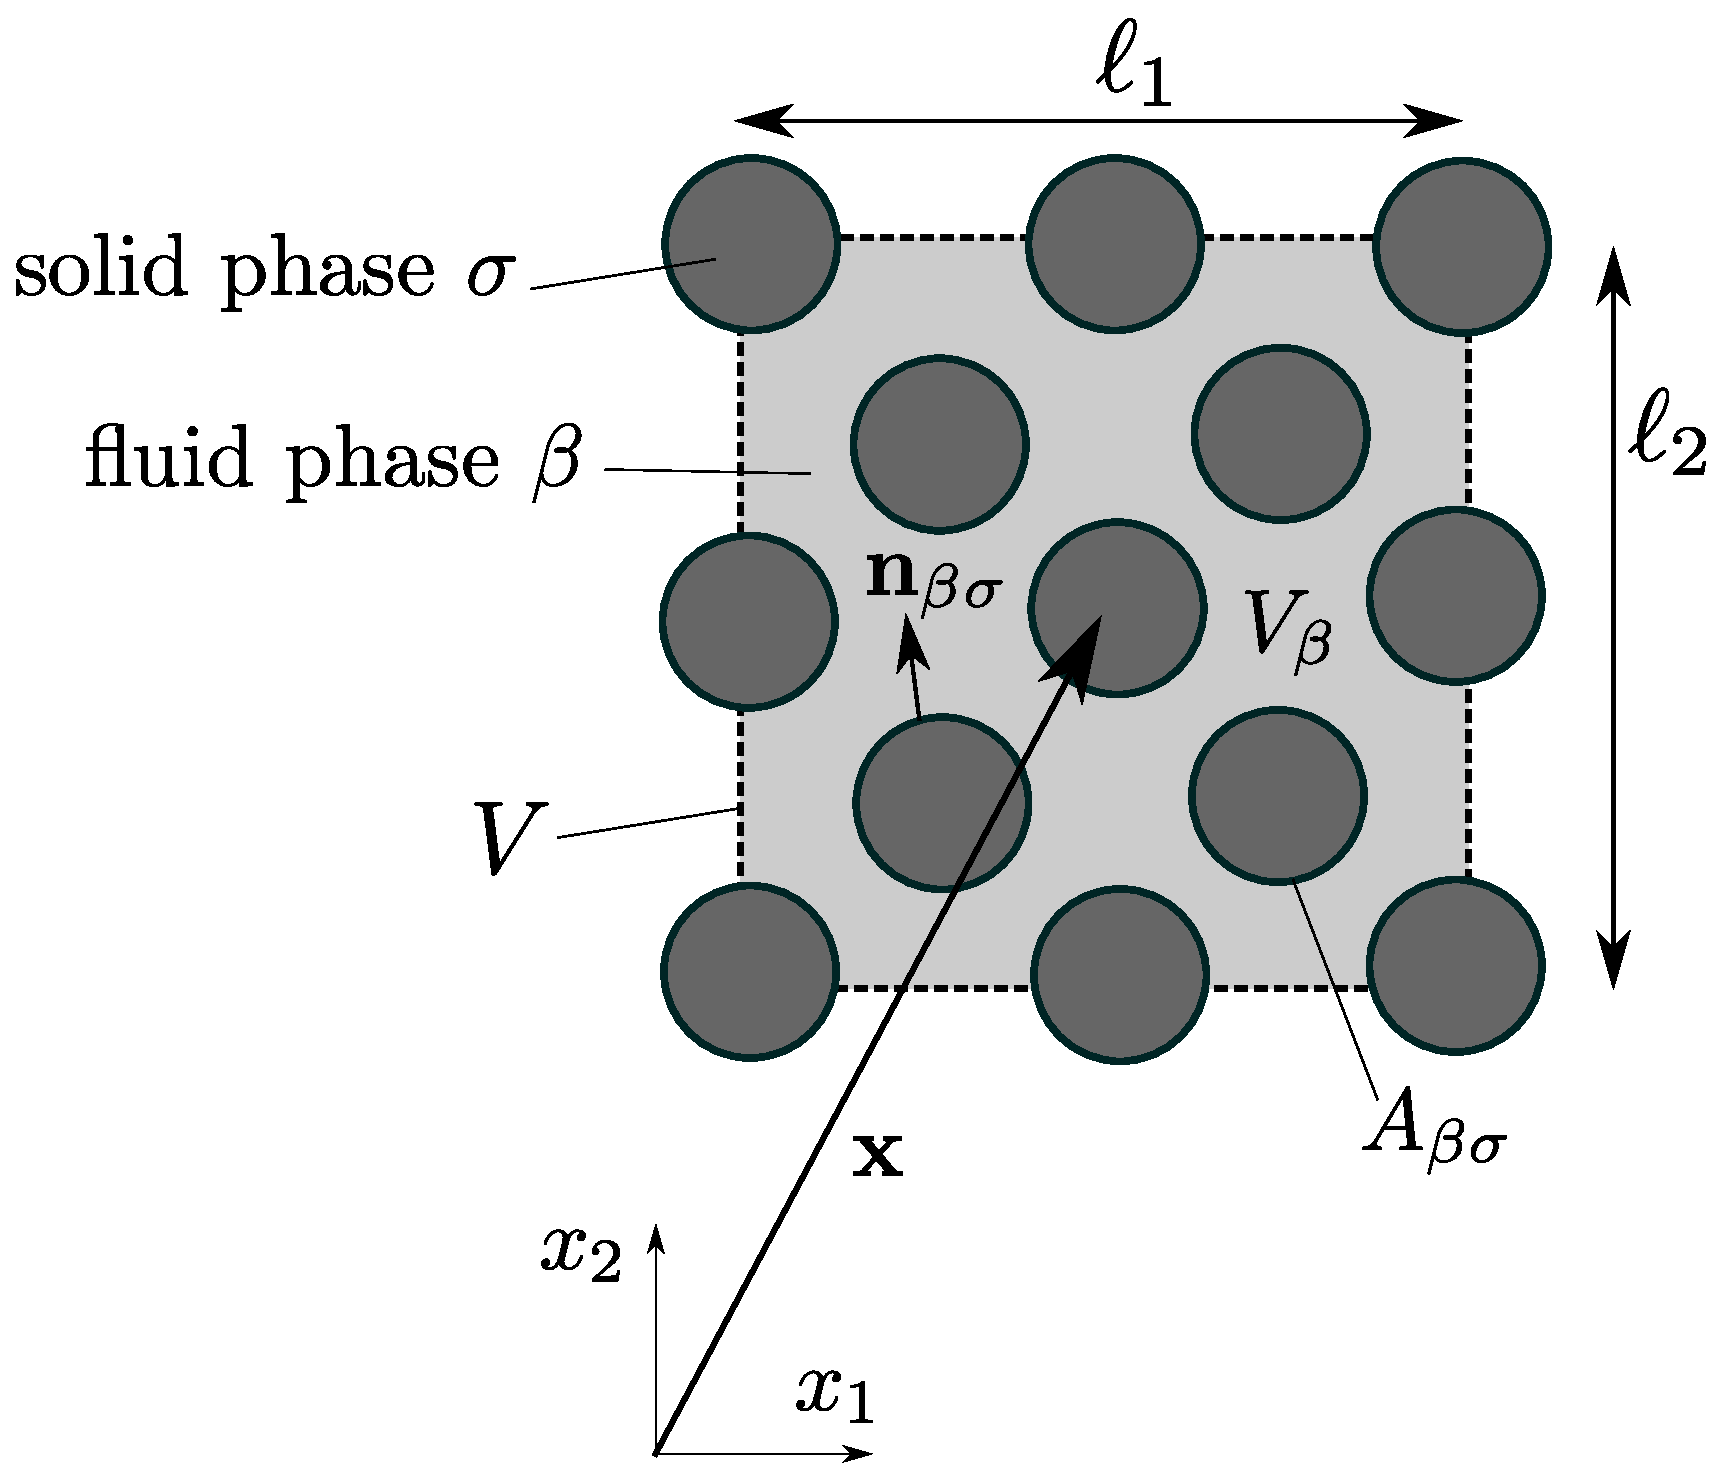
\includegraphics[width=0.8\linewidth]{chapter_4/figure/REV}
%	\caption{Illustration of the REV concept.}
%	\label{fig:rev}
%\end{figure}
%
%
%The concept of Reference Elementary Volume (REV) of the porous medium is classically introduced in the framework of the VANS approach.
%An example of REV  is depicted on figure \ref{fig:rev}, together with relevant notations (volume shape and size, indication of the fact that the normal unit vector is directed from the fluid to the solid phase, centroid $\rm {\bf{x}}$ of the REV). The REV represents  the domain over which the    microscopic problem is solved; its size is defined so as to contain all the microscopic features of the flow. 
%As a rule of thumb, the REV is the smallest  fluid domain over which   periodic boundary conditions can be applied.
%
%
%In the computational domain, any flow variable  $\phi$ can be decomposed into an intrinsic average part $\meani{\phi}$ plus a perturbation $\tilde{\phi}$, as:
%$$  \phi = \meani{\phi} + \tilde{\phi}.$$
%The intrinsic average is defined with an integration carried out only on the fluid phase \cite{whitaker2013method}:
%\begin{equation}
%\meani{\psi_{\beta}} = \dfrac{1}{\volb} \int_{\volb} \psi_\beta (\mathbf{x}) d \volb.
%\label{eq:avg_intrinsic}
%\end{equation}
%Applying such an operator to equations \eqref{eq:mom} and \eqref{eq:cont}, and following \citet{whitaker1996forchheimer} we have:
%$$
%\dfrac{\partial \vbmi}{\partial t} + \vbmi \cdot \nabla \vbmi = -\frac{1}{\rho_{\beta}} \nabla \pbmi + \nu_\beta \nabla^2 \vbmi + \, \mathbf{f} \, + 
%$$
%\begin{equation}
%\dfrac{1}{\volb} \int_{A_{\beta \sigma}}  ( - \frac{\pbt}{\rho_\beta} \mathbf{I} + \nub \nabla \vbt ) \cdot  \mathbf{n}_{\beta \sigma} dA,
%\label{eq:darcy_forch}
%\end{equation}	
%\begin{equation}
%\nabla \cdot \meani{\vb} = 0,
%\label{eq:cont_vans}
%\end{equation}	
%upon neglecting in equation \eqref{eq:darcy_forch} the sub-REV scale dispersion term (linked to the $\left< \vbt \vbt \right>^{\beta}$ term) which is often small in porous media flows \cite{brugem_phd}.
%
%The surface integral term in equation \eqref{eq:darcy_forch}  represents the drag (per unit mass) due to surface forces at the fluid-solid interface of the medium. It is called the Darcy-Forchheimer microscale force, $\mathbf{F}^{\textit{m}}$. The equations are however often to be solved at the macroscale, so that a macroscale force model, 
%$\mathbf{F}^{\textit{M}}$, must be used to replace $\mathbf{F}^{\textit{m}}$ in the governing equation. Such a model is often based on a permeability tensor, $\mathbf{K}$, and a Forchheimer tensor, $\mathbf{F}$, and reads:
%\begin{equation} 
%\mathbf{F}^{\textit{M}} = - \nub \mathbf{K}^{-1} (\mathbf{I} + \mathbf{F})\vbmi,
%\label{eq:macroscale} 
%\end{equation}
%so that the system is closed by imposing
%\begin{equation}
%\mathbf{F}^{\textit{m}} = \mathbf{F}^{\textit{M}}.
%\label{eq:closure_KF} 
%\end{equation}
%
%
%\noindent The drag force $\mathbf{F}^{\textit{m}}$ computed by direct numerical simulations (DNS) with account of all individual pores will be later compared to the model based on the permeability and Forchheimer tensors (whose equations are given below).
%This is just a useful exercise to demonstrate consistency of the approach and accuracy of the numerical simulations; it does nothing else since, as briefly described below, to derive the Forchheimer tensor the microscopic velocity field must be known anyhow.  Nonetheless, knowledge of the behaviour of these tensors (or, equivalently, of the related \emph{apparent} permeability) might prove both useful and instructive, in particular should one wish to extend the range of applicability of the model to cases for which the microscopic solution is not available.
%
%
%
%%%%%%%%%%%%%%%%%%%%%%%%%%%%%%%%%%%%%%%%%%%%%%%%%%%%%%%%%%%%%%
%%
%%\subsubsection{Closure problems for $\mathbf{K}$ and $\mathbf{F}$}
%%
%%%%%%%%%%%%%%%%%%%%%%%%%%%%%%%%%%%%%%%%%%%%%%%%%%%%%%%%%%%%%%
%
%
%The core of the VANS approach consists in the identification of the permeability and Forchheimer tensors. This problem, referred to as the closure problem, is discussed at length by \citet{whitaker1986flow,whitaker1996forchheimer}.  He derives two partial differential equation systems, the first valid in the zero Reynolds number limit (system \eqref{eq:K_closure} below), while the second applies when inertial terms are not negligible (system \eqref{eq:F_closure1}).
%
%
%
%In the first system of equations   a three component vector $\mathbf{d}$  and  a $3 \times 3$ tensor  $\mathbf{D}$ are introduced.
%This system  can be divided into  three separate independent problems which resemble a forced Stokes problem where each component of $\mathbf{d}$ and the corresponding row of  $\mathbf{D}$  play, respectively, the role of a pressure and a velocity field. Together with the periodic  boundary conditions, the problem reads: 
%\begin{equation}
%\begin{cases} 
%0 = -\nabla \mathbf{d} + \nabla^2 \mathbf{D} + \mathbf{I},\\ 
%\nabla \cdot \mathbf{D} = 0, \\ 
%\mathbf{D} = 0 \qquad {\rm on }  \qquad A_{\beta \sigma},\\
%\mathbf{d}(\mathbf{x} + \ell_i) = \mathbf{d}(\mathbf{x}), \qquad 
%\mathbf{D}(\mathbf{x} + \ell_i) = \mathbf{D}(\mathbf{x}) \qquad i = 1,2,3.
%\end{cases} 
%\label{eq:K_closure}
%\end{equation}
%The permeability tensor is found by applying  the intrinsic average on the $\mathbf{D}$ tensor, i.e.
%$\mathbf{K} = \varepsilon \; \meani{\mathbf{D}}$  and, in the Stokes regime, it is
%\begin{equation}
%\mathbf{F}^{\textit{M}} = - \nub \mathbf{K}^{-1} \vbmi.
%\end{equation}
%
%The second closure problem differs from the first only for the presence of a linearised convective term 
%in which the microscopic velocity obtained from the DNS, $\vb$, is used as an input.  This of course implies knowledge of the microscopic velocity field. A Oseen-like approximation which relaxes this constraint has been proposed by \citet{zampogna}.
%
%The new unknowns are a  vector and a tensor called, respectively,   $\mathbf{m}$  and  $\mathbf{M}$, with  the same meanings of $\mathbf{d}$ and 
%$\mathbf{D}$.
%The system reads:
%\begin{equation}
%\begin{cases} 
%\dfrac{1}{\nub} \vb \cdot \nabla \mathbf{M} = -\nabla \mathbf{m} + \nabla^2 \mathbf{M} + \mathbf{I},\\ 
%\nabla \cdot \mathbf{M} = 0, \\ 
%\mathbf{M} = 0  \qquad {\rm on } \qquad A_{\beta \sigma}, \\
%\mathbf{m}(\mathbf{x} + \ell_i) = \mathbf{m}(\mathbf{x}), \qquad 
%\mathbf{M}(\mathbf{x} + \ell_i) = \mathbf{M}(\mathbf{x}) \qquad i = 1,2,3.
%\end{cases} 
%\label{eq:F_closure1}
%\end{equation}
%The average  of the tensor $\mathbf{M}$  multiplied by the porosity is the \textit{apparent permeability}, 
%$\mathbf{H}= \varepsilon \; \meani{\mathbf{M}}$. When inertia is important equation \eqref{eq:macroscale}  can be written as 
%\begin{equation}
%\mathbf{F}^{\textit{M}} = - \nub \mathbf{H}^{-1} \vbmi,
%\end{equation}
%\noindent as shown by \citet{whitaker1996forchheimer}.
%
%Two remarks are in order at this point.
%First, the equations in the closure problem \eqref{eq:F_closure1} are time-independent because the microscopic velocity $\vb$ is a solution of a stationary DNS.  Thus, the Reynolds number should be sufficiently small for unsteady effects not to be present. Should the wake behind a solid inclusion display regular or irregular temporal oscillations, the equations of system \eqref{eq:F_closure1} may be used, as an
%approximation, by replacing the instantaneous velocity in the REV with its time-averaged distribution.  This case is however not of present concern.
%Secondly, the closure problems reflect the structure of the solution of the two system \eqref{eq:K_closure} and \eqref{eq:F_closure1}. In particular, the solution of \eqref{eq:K_closure} depends only on the geometry of the porous medium so that the permeability tensor $\mathbf{K}$ is symmetric. This is not the case for $\mathbf{H}$, because of the effect of the microscopic velocity amplitude and direction.  Clearly, the solution of system \eqref{eq:K_closure} tends to that of \eqref{eq:F_closure1} when $Re_d \rightarrow 0$. 
%



%%%%%%%%%%%%%%%%%%%%%%%%%%%%%%%%%%%%%%%%%%%%%%%%%%%%%%%%%%%%%%

\section{Validation and setup }

%%%%%%%%%%%%%%%%%%%%%%%%%%%%%%%%%%%%%%%%%%%%%%%%%%%%%%%%%%%%%%%


In this section the numerical methodology, the parameters, the setup and the validation for some reference cases are given.


%%%%%%%%%%%%%%%%%%%%%%%%%%%%%%%%%%%%%%%%%%%%%

\subsection{Computational domain}

%%%%%%%%%%%%%%%%%%%%%%%%%%%%%%%%%%%%%%%%%%%%%


The geometry used for the base REV is shown in figure \ref{fig:cell_3d}: a cylindrical inclusion is present at the centre of the REV and four quarters of cylinders are situated at the corners. The lateral length of the cubic envelop is $\ell$, which is used as length scale for the microscopic problem; the diameter $d$ of the cylinders is adapted as a function of the desired porosity $\varepsilon$, ratio between the fluid volume over the total REV volume ($\ell^3$). 

The  forcing term $\mathbf{f}$ of the DNS  is a vector whose direction is defined by two Euler angles, with rotations of the form:  $\theta \ \mathbf{e_3} + \phi \ \mathbf{e_2}^{I}$ (cf. figure \ref{fig:cell_3d}). Its amplitude is set a priori and is connected to the Reynolds number, $Re_d$, defined with the mean velocity over the REV and the fiber diameter, $d$. $Re_d$ is a result of the calculations, once the mean velocity is evaluated.

\begin{figure}[h]
	\centering
	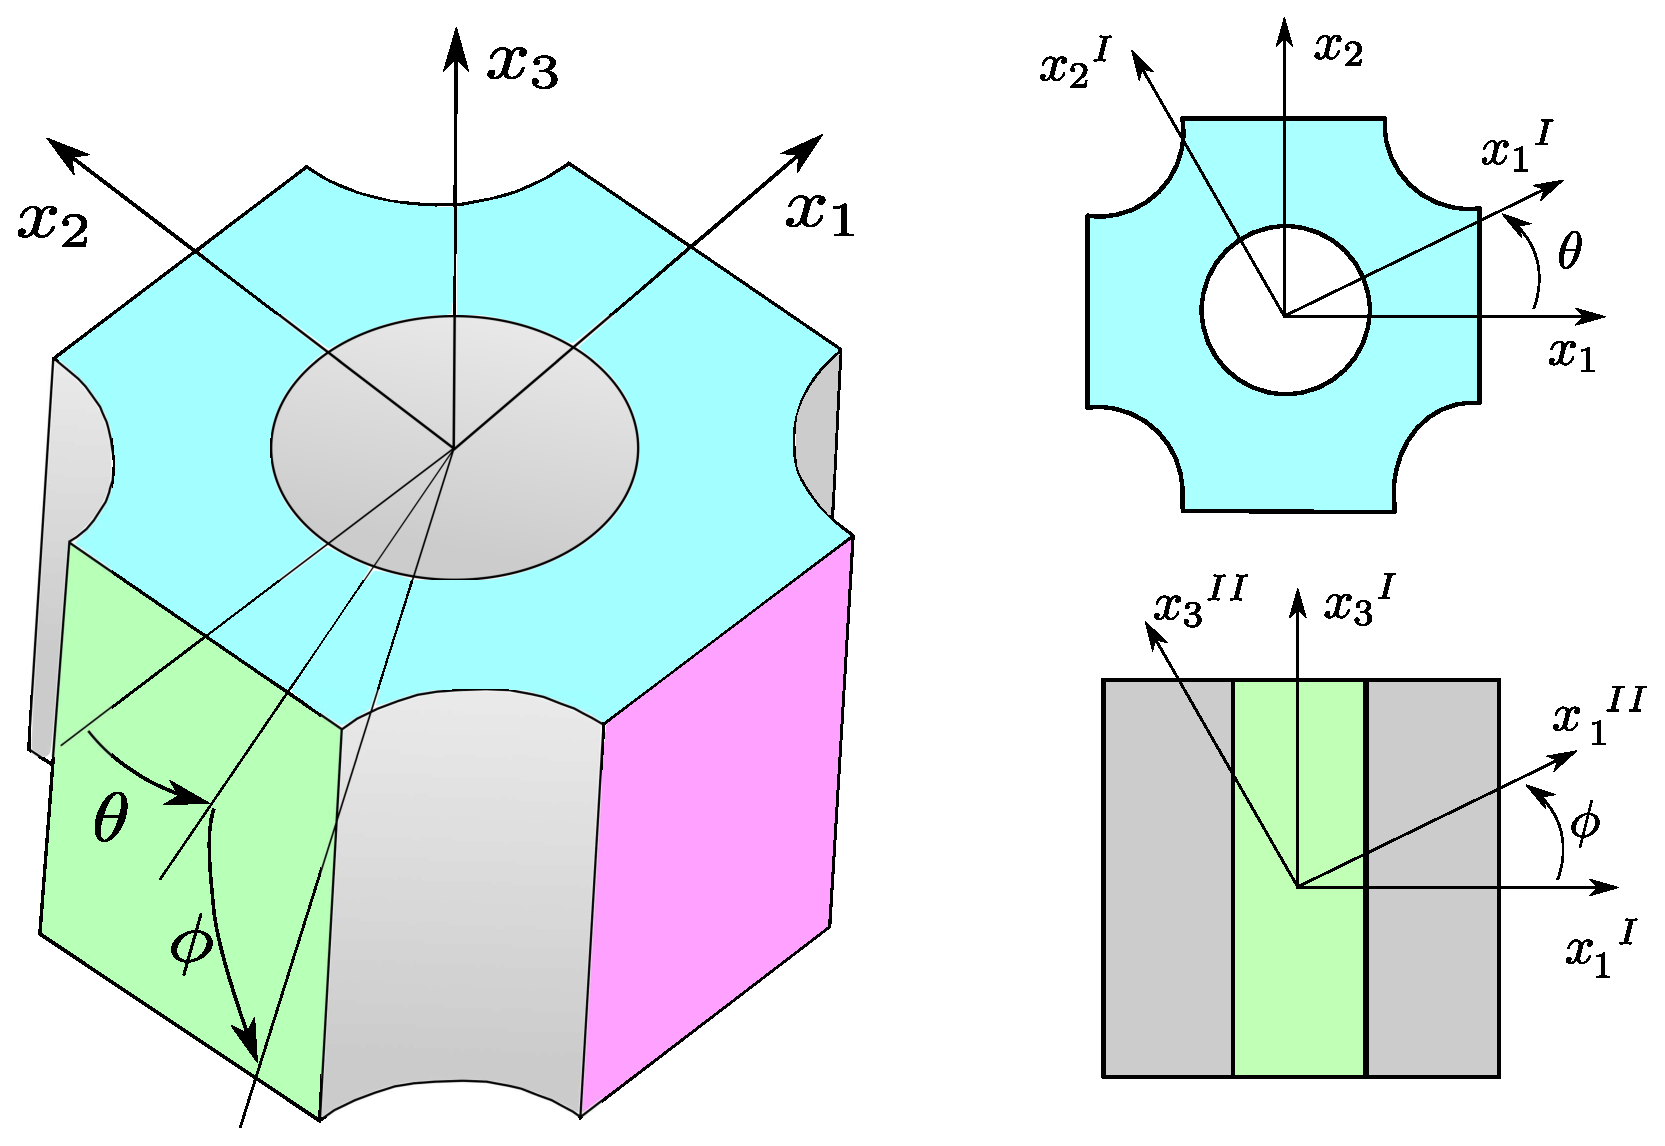
\includegraphics[width=0.8\linewidth]{chapter_4/figure/cell_3d}
	\caption{REV for the fiber geometry investigated.}
	\label{fig:cell_3d}
\end{figure}


%%%%%%%%%%%%%%%%%%%%%%%%%%%%

\subsection{Numerical setup}

%%%%%%%%%%%%%%%%%%%%%%%%%%%%


The simulations have been carried out with the open-source code OpenFOAM \cite{openfoam}, based on  a finite volume discretization with a colocated arrangement for the unknowns.
The standard solver icoFoam (incompressible Navier-Stokes) has been modified in order to include a constant pressure gradient acting as a forcing term $\mathbf{f}$  in equation \eqref{eq:mom}. 
The coupling between  the velocity and the pressure equations is based on the pressure implicit split operator referred to as the PISO algorithm. 
The time derivative term is discretized using the second order backward Euler scheme and all the spatial terms use a second-order central difference stencil  based on Gauss finite volume approach. The velocity system is solved with a preconditioned bi-conjugate gradient (PBiCG) iterative solver with the tolerance on the velocity residuals set to $10^{-8}$, associated to a   diagonal incomplete lower upper pre-conditioner (DILU).
The pressure equation is solved with a  geometric-algebraic multigrid  (GAMG) algorithm associated to a Gauss-Seidel smoother and the tolerance on the pressure residuals is here equal to $10^{-6}$.  Cyclic boundary conditions are applied to all fields on all fluid
boundaries along the three directions, and the no-slip condition is imposed on the surface of the solid inclusions. 
The time step $\Delta t$  is automatically determined to ensure  that the maximum Courant number, $Co$, respects the condition:
$Co =  ||v_\beta||  \ \Delta t / \Delta x < 1/2 $, in which $||v_\beta||$ is the local velocity magnitude in the REV and $\Delta x$ is the local grid spacing. $Co$ 
is basically the ratio between the fluid speed  and the velocity to propagate information through the mesh and the condition $Co < 1/2$ is found to be sufficient to have a stable solver.



%%%%%%%%%%%%%%%%%%%%%%%%%%%%%%%%%%%%%%%%

\subsection{Mesh convergence analysis }

%%%%%%%%%%%%%%%%%%%%%%%%%%%%%%%%%%%%%%%%


The mesh has been computed using  the internal OpenFOAM mesher named \textit{snappyHexMesh}.
The final grid is mainly composed by hexahedral cells with a refined regular grid in the boundary layer regions next to the solid surfaces.
Three different mesh sizes, with $0.65 \times 10^6$, $10^6$ and $1.5 \times 10^6$ elements, have been tested in order to demonstrate spatial convergence. This has been assessed using the Grid Convergence Index ($GCI$) introduced by \citet{roache}.



Details of the coarsest mesh used are shown in figure \ref{fig:mesh1}. On the  right frame a close up of the grid in the neighbourhood of the fiber's boundary is displayed: twenty points are used in the structured portion of the mesh along the wall-normal direction.



\begin{figure}[h]
	\centering
	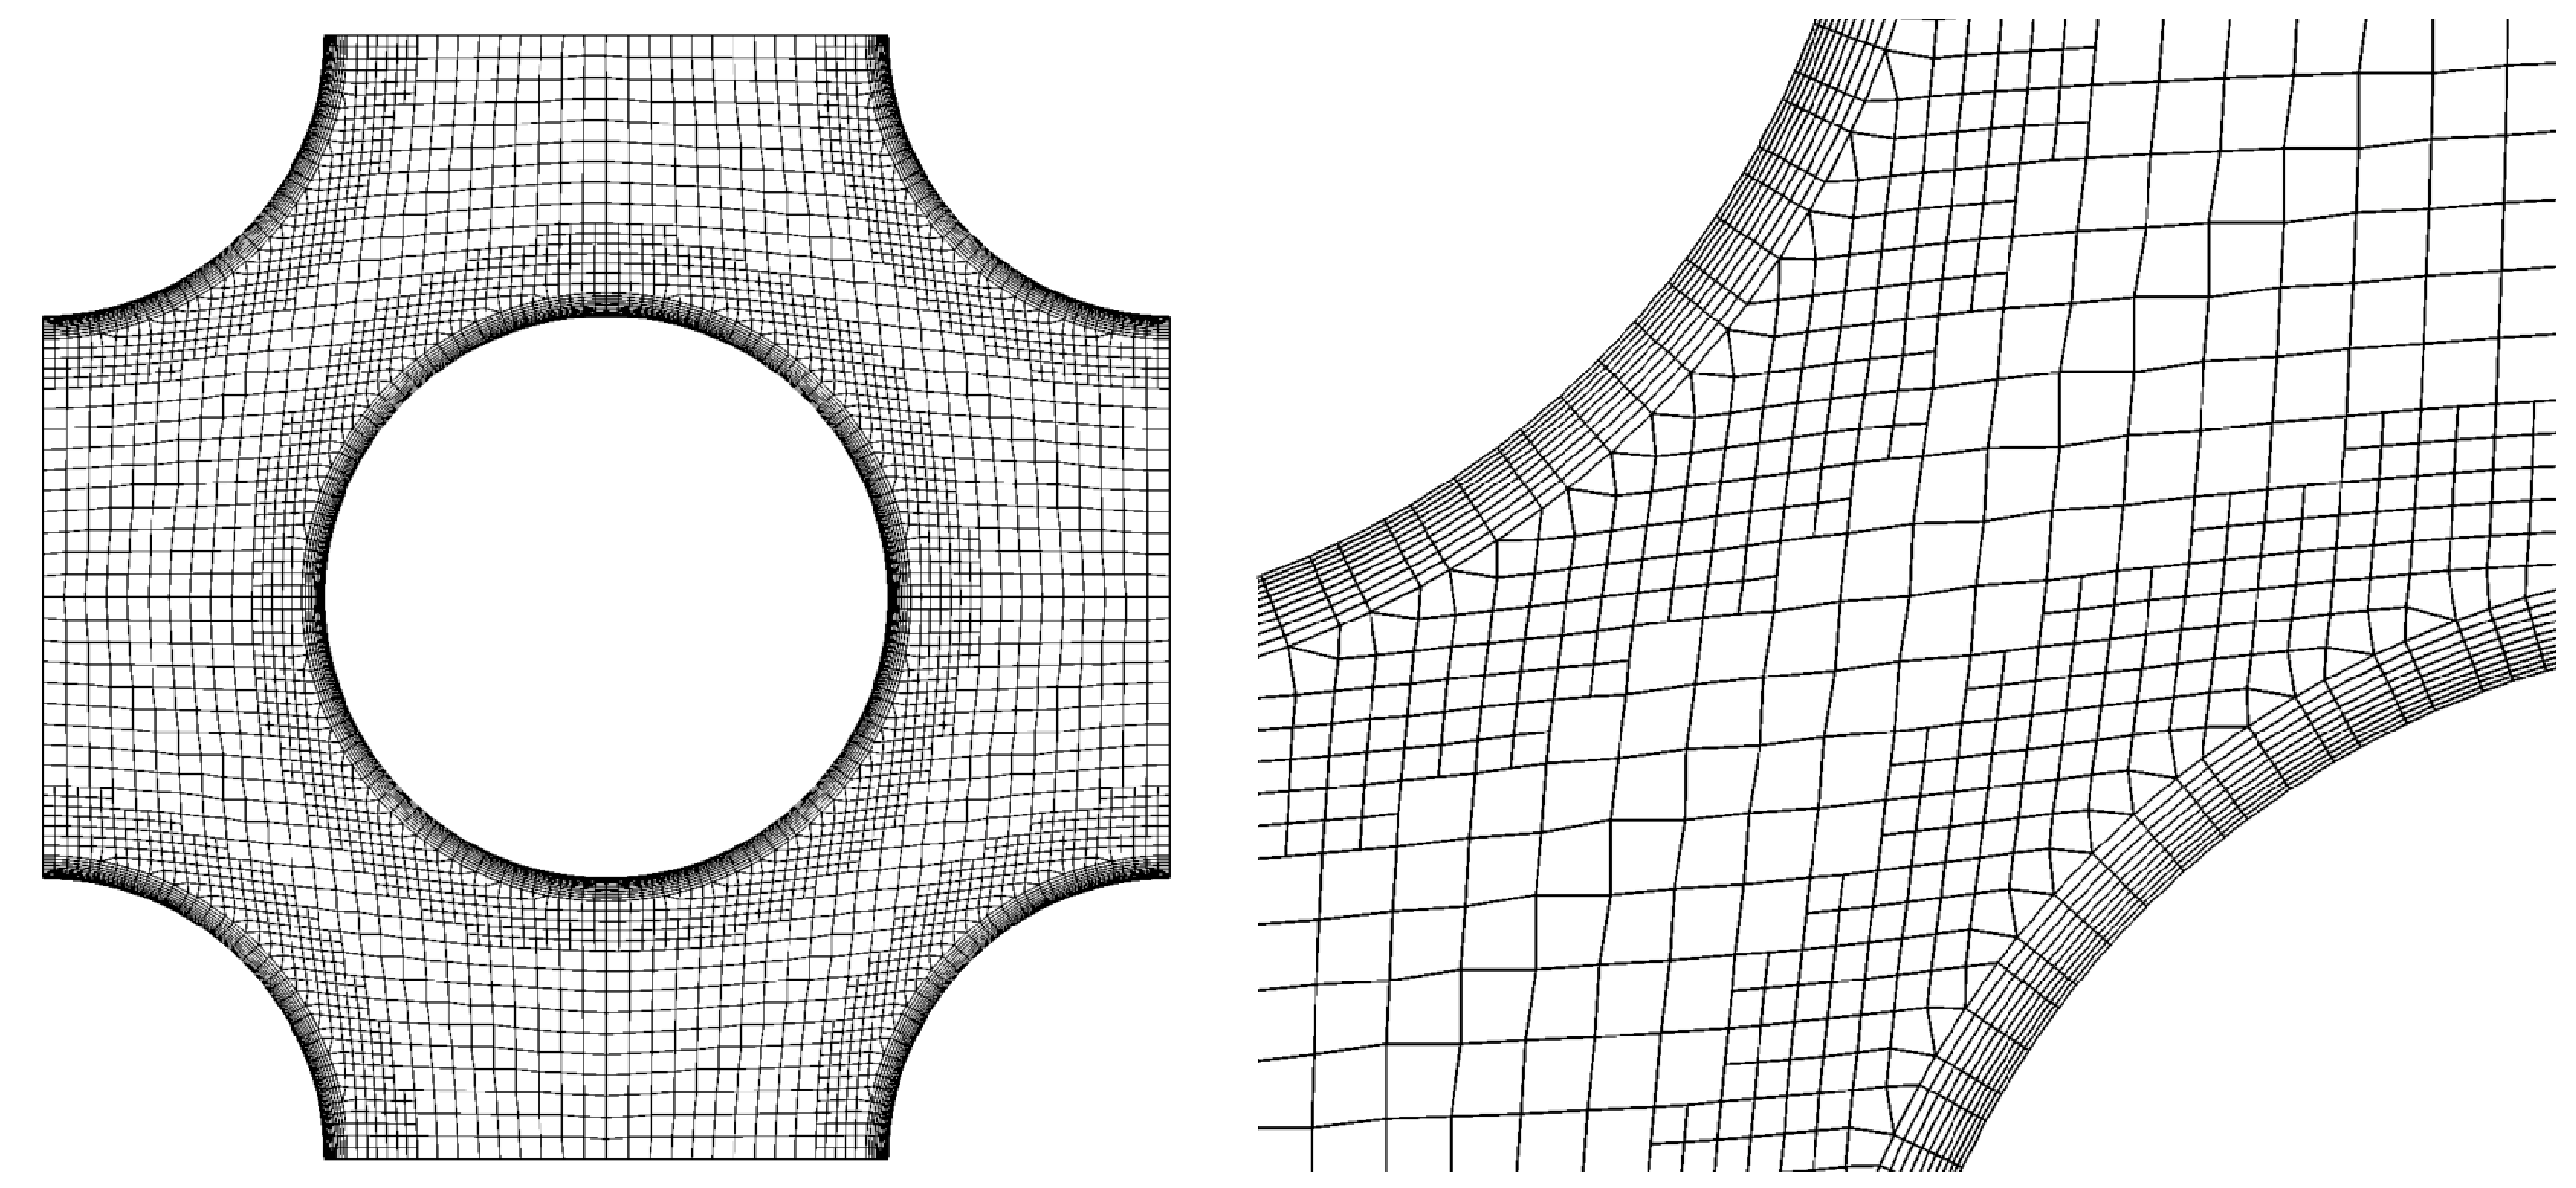
\includegraphics[width=0.8\linewidth]{chapter_4/figure/mesh}
	\caption{Mesh used for the computation; top view (left) and zoom in the boundary layer region (right). $\varepsilon = 0.6$.}
	\label{fig:mesh1}
\end{figure}




The GCI method is based upon a grid refinement error estimator derived from the
theory of generalized Richardson extrapolation. It measures the ratio between the computed value of a quantity over the asymptotic numerical value, thus indicating how far the solution is from the asymptotic ("exact") value.
The procedure is simple and provides a method to estimate the order of the spatial
convergence, based on two or three different grid sizes.
First of all, the grids must be generated with the same algorithm and they must  have the same final quality.
In each simulation   a physical scalar quantity representative of the physical phenomenon must be sampled.
The method follows the following four steps:

\begin{enumerate}
	\item  Estimate the order of convergence of the procedure, defined as
	$p = \ln \rprth{\dfrac{f_3 - f_2}{f_2 - f_1}}   / \ln r $,
	where $r$ is the grid refinement ratio between each grid (it is computed as the ratio between the number of elements of two consecutive grids; the approach imposes that $r$ should remain constant between any couple of consecutive grids and be larger than $1.1$), and $f_i$
	represents the quantity of interest in each grid (1=coarse, 2=medium and
	3=fine).
	
	
	\item Compute the relative error between grid $i$ and $j$:
	${|\epsilon|}_{ij} = \dfrac{f_j - f_i}{f_i}$, for $(i,j)$
	$\in \left\{ (1,2), (2,3) \right\}$.
	
	\item Compute
	$ {GCI}_{ij}=\dfrac{F_s {|\epsilon|}_{ij}}{r^p -1}$, with
	$F_s$ a safety factor equal to 1.25 if the grids are three, and equal to 3 if the grids are only two \cite{roache}.
	
	\item Check whether each grid level yields a solution that is in the asymptotic range of convergence; this means that the quotient
	$ AC = \dfrac{{GCI}_{23}}{{GCI}_{12}} \dfrac{1}{r^p}$ should be as close as possible to one.
\end{enumerate}


\noindent In our case the quantity of interest chosen is the intrinsic average velocity inside the porous medium, and the results are summarized in table \ref{table:convergence}.
\begin{table}[t]
	\begin{center}
		\begin{tabular}{ l  |l   l   }
			\vspace{-0.3cm}
			mesh   &	mesh   & average REV  \\
			index  &	identifier  &  velocity \\ 
			\hline \hline
			3 &	fine & 1.11  \\ 
			2 &	medium & 1.07  \\ 
			1 & coarse & 1.09  \\ 
			\hline
		\end{tabular}
		$\qquad$
		\begin{tabular}{ l | l   }\vspace{0.35cm} 
			metric & value \\ \hline \hline
			${GCI}_{23}$ & 0.366\%  \\ 
			${GCI}_{12}$ & 1.11\%  \\ 
			AC & 1.006  \\
			\hline
		\end{tabular}
		\caption{Convergence analysis. Left: average velocity within the REV, normalized with $\displaystyle{\frac{K_{11}}{\nu_{\beta}} ||\bf{f}||}$. 
			Right: grid convergence metrics. The REV has $\varepsilon=0.6$, the motion is along $x_1$, i.e. 
			$\theta=\phi=0$ and $Re_d \rightarrow 0$.}
		\label{table:convergence}
	\end{center}
\end{table}
From the table it can be seen that the intrinsic velocity difference is very small from one grid to the next and the coarse grid provides results close to the expected asymptotic value. This is taken as a sufficiently convincing argument to carry out all the computations in the following with a grid density equal to that of grid 1. 



%%%%%%%%%%%%%%%%%%%%%%%%%%%%%%%%%%%%%%%%%%%%%%%%%%%%%%%
\subsection{Validation on two different configurations}
%%%%%%%%%%%%%%%%%%%%%%%%%%%%%%%%%%%%%%%%%%%%%%%%%%%%%%

The results published in the literature by \citet{zampogna} and \citet{yazdchi2011} are now used to validate both the methodology and our choices of the computational parameters. In the cited papers, three-dimensional  computations of the permeability components in different cells geometries are presented.

Figure \ref{fig:square} displays the comparison for a cell with a square arrangements  of the fibers; here the permeability is evaluated along the two principal directions, $x_1$ and $x_3$.
%The present computation are plot with triangles for the two $K_{11}$ and $K_{33}$ components.
A good agreement is found with the published results. 
%For permeability $\varepsilon$ larger than $0.85$, some small discrepancies can be seen but it is at the limit of the theory.
%The trends are well captured as well by comparison with the empirical fitted solution given by the reference.
\begin{figure}[t]
	\centering
	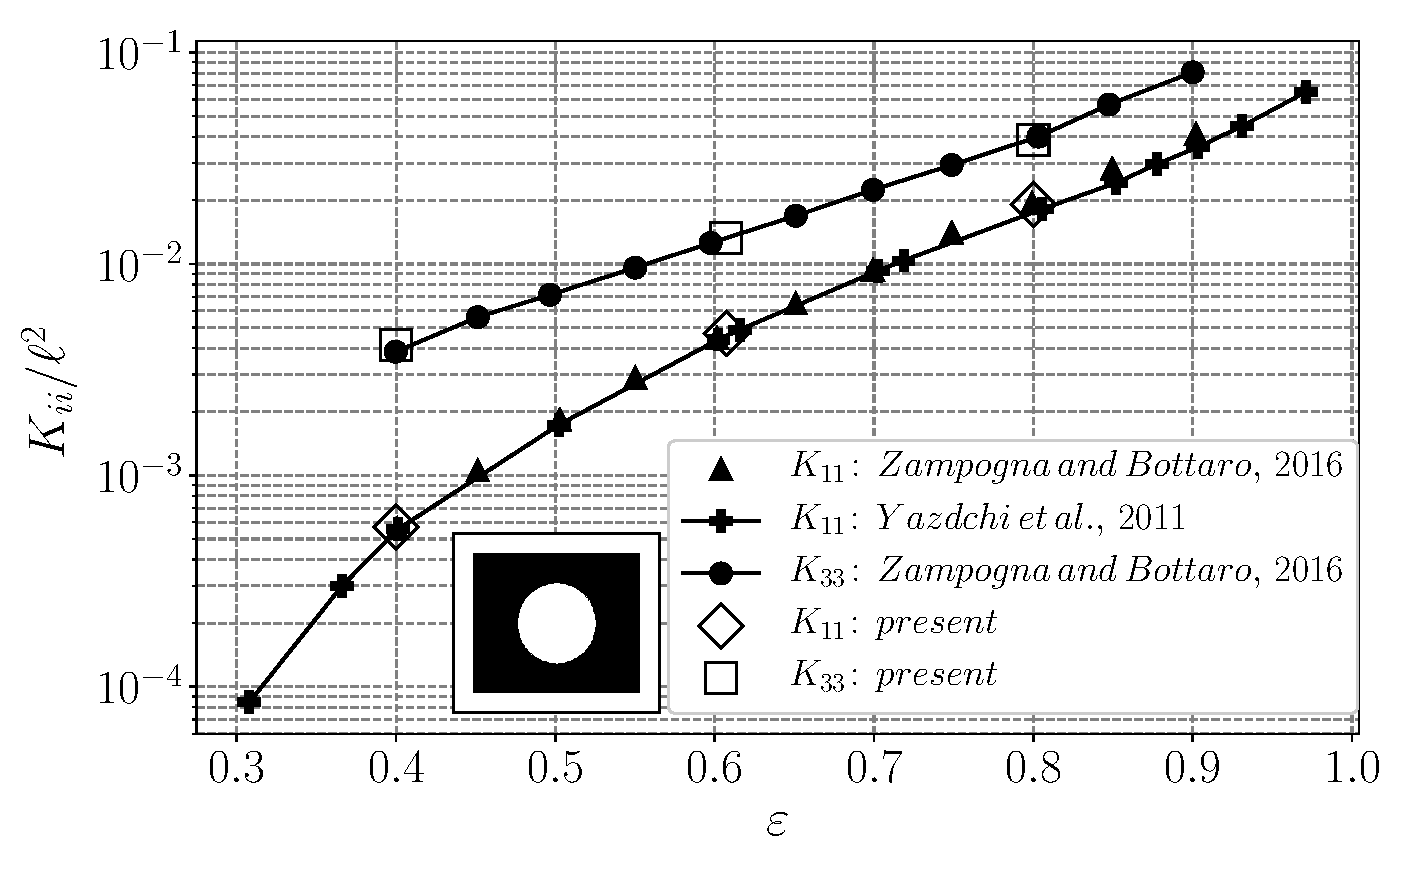
\includegraphics[width=0.8\linewidth]{chapter_4/figure/square}
	\caption{Permeability versus porosity for a square arrangement of cylinders. The scaling of the permeability is $\ell^2$ and is explicitely indicated in the vertical axis.}
	\label{fig:square}
\end{figure}
Figure \ref{fig:hexa} shows a similar comparison for a staggered arrangement of the inclusions in the unit cell. In this case the section of the cell is rectangular. The agreement for the only permeability component available in the literature is again satisfactory.
\begin{figure}[h]
	\centering
	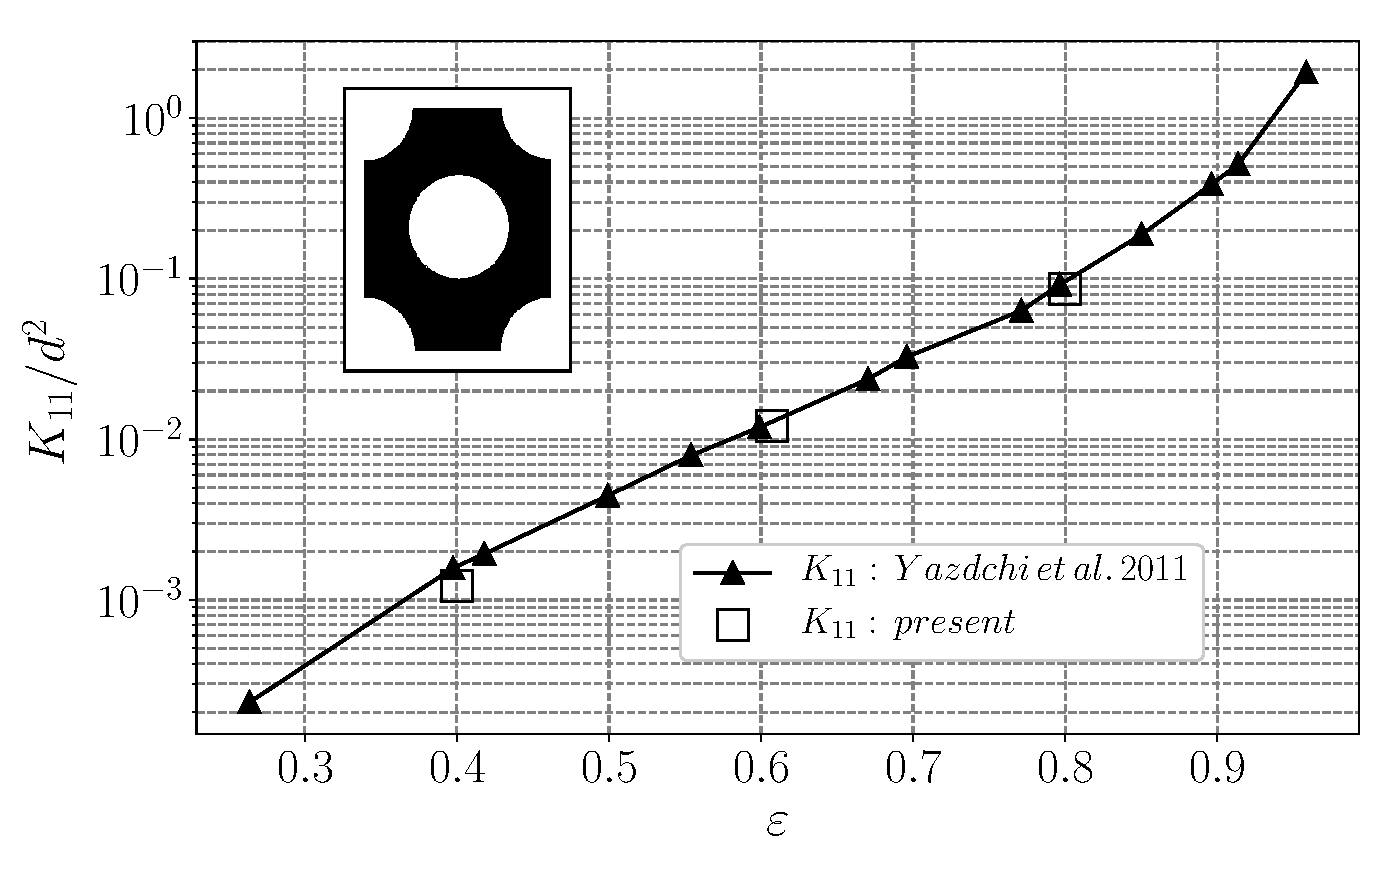
\includegraphics[width=0.8\linewidth]{chapter_4/figure/hexa}
	\caption{Permeability versus porosity for a staggered arrangement of cylinders. The permeability component is here scaled with $d^2$ (and not $\ell^2$), with $d$ the diameter of the inclusions.}
	\label{fig:hexa}
\end{figure}

\begin{figure}[h!]
	\centering
	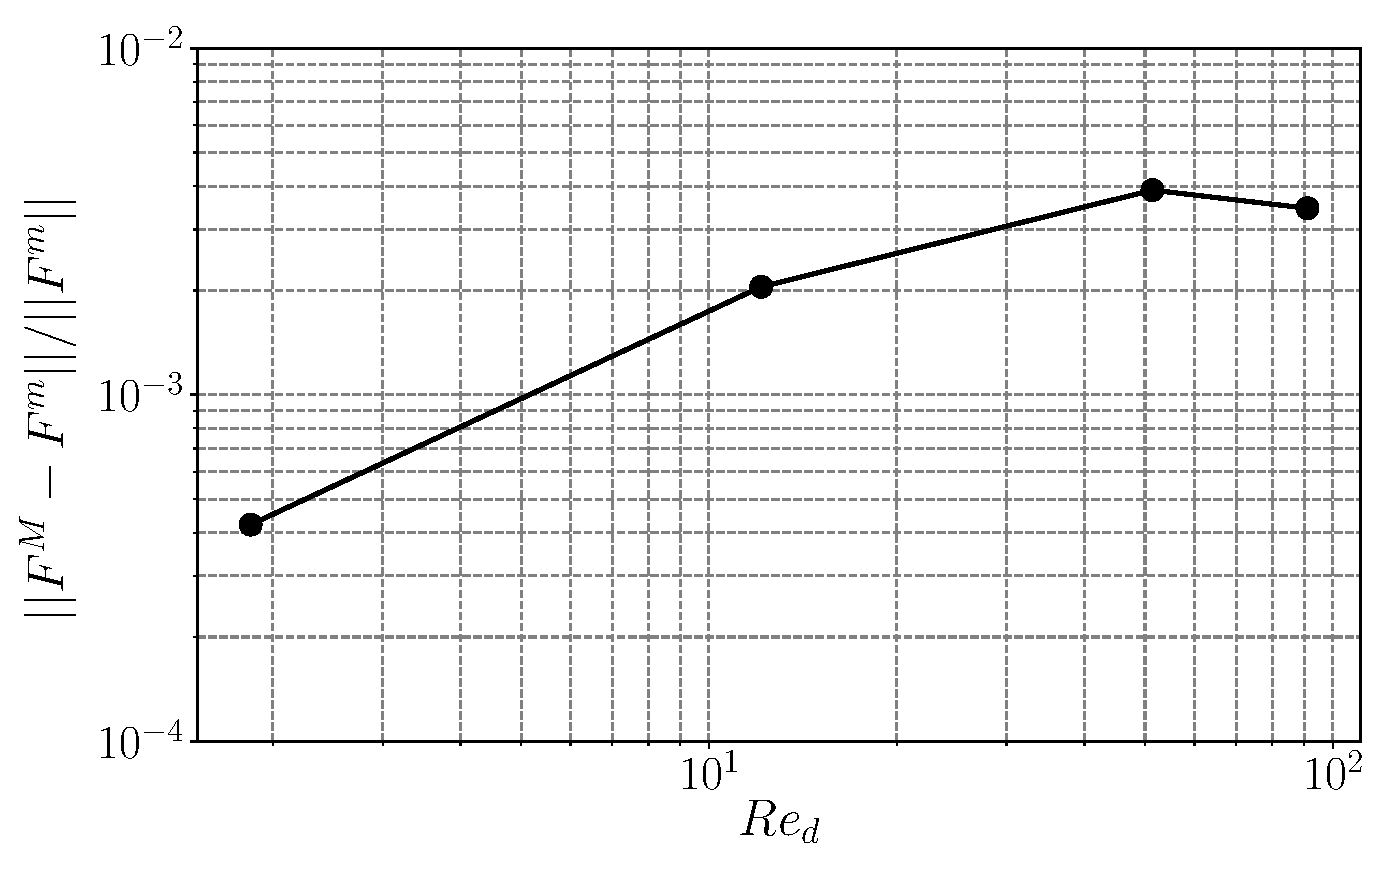
\includegraphics[width=0.8\linewidth]{chapter_4/figure/macro_force}
	\caption{Relative error between the microscopically computed forces along the $x_1$ direction and those arising from the Darcy-Forcheimmer model; $\varepsilon=0.8$ for the REV in the staggered arrangement of \citet{yazdchi2011}.}
	\label{fig:force_comparison}
\end{figure}	
Finally, to check the correct implementation of the closure model \eqref{eq:closure_KF} it is important to verify the equality \eqref{eq:closure_KF}  between the amplitude $F^M$ of the macroscopic force and its microscopic counterpart obtained through an integration of the DNS fields over the solid boundaries of the inclusions in the REV. Figure \ref{fig:force_comparison} shows a plot of the relative error between these two forces, i.e. 
$\displaystyle \frac{||F^M-F^m||}{||F^m||}$, as function of the Reynolds number. We consider the successful comparison displayed in figure \ref{fig:force_comparison} 
as the conclusive demonstration of the validity of the approach described here. We have nonetheless carried out the same verification displayed in figure \ref{fig:force_comparison} for each one of the simulations described in the following, to our satisfaction.



%%%%%%%%%%%%%%%%%%%%%%%%%%%%%%%%%%%%%%%
\subsection{Tests with larger REV's}
%%%%%%%%%%%%%%%%%%%%%%%%%%%%%%%%%%%%%%%

Since the Reference Elementary Volume (REV) is the unit cell within the porous medium over which average quantities of the VANS are computed, 
it is important to choose its dimensions appropriately in the inertial regime for, if the REV is too small, it might be easy to miss crucial 
features of the wakes. For example, to predict the  critical Reynolds number, $Re_c$, of the first Hopf bifurcation, a REV containing at least 
three solid inclusions in the direction of the mean pressure gradient is necessary in the simulations by \citet{lasseux_hopf}. Among the 
results 
reported, it is found that, for a fixed REV size, the error committed in the evaluation of the critical Reynolds number increases with the 
porosity. This same error is considerably reduced when the mean pressure gradient angle is $\theta=45^\circ$. Thus, the choice of the number of 
inclusions in a REV is a task not to be overlooked, and the final choice must account for the porosity, the direction of the pressure gradient 
and the microscopic Reynolds number.

Here, the influence of the numbers of inclusions present in a REV is assessed by focussing only on the velocity components after averaging over the REV. The unit cubic cell of side $\ell$ is used as reference: starting from this, two additional REV's are built, as shown in figure \ref{fig:multiple}. The first one is doubled in both the $x_1$ and $x_2$ directions and the case tested numerically is characterised by $\theta=0$, $\phi=0$ (i.e. the forcing pressure gradient is directed along $x_1$), porosity $\varepsilon=0.6$ and $Re_d=50$. 
The second REV configuration is a composition of 3 reference REVs on top of one another along $x_3$, with the parameters set to $\theta=45^\circ$, $\phi=45^\circ$,  $\varepsilon=0.6$ and $Re_d=100$.

For both these test cases, no appreciable differences, neither in the mean velocity nor in the forces on the fibers, have been observed, with relative errors on the mean velocity with respect to the reference case which remain below  2\%.  We take this as sufficient evidence to use, in the following, only the reference cubic REV of side equal to $\ell$, with the understanding that only configurations with $Re_d$ up to around 100 can be considered.

\begin{figure}[h!]
	\centering
	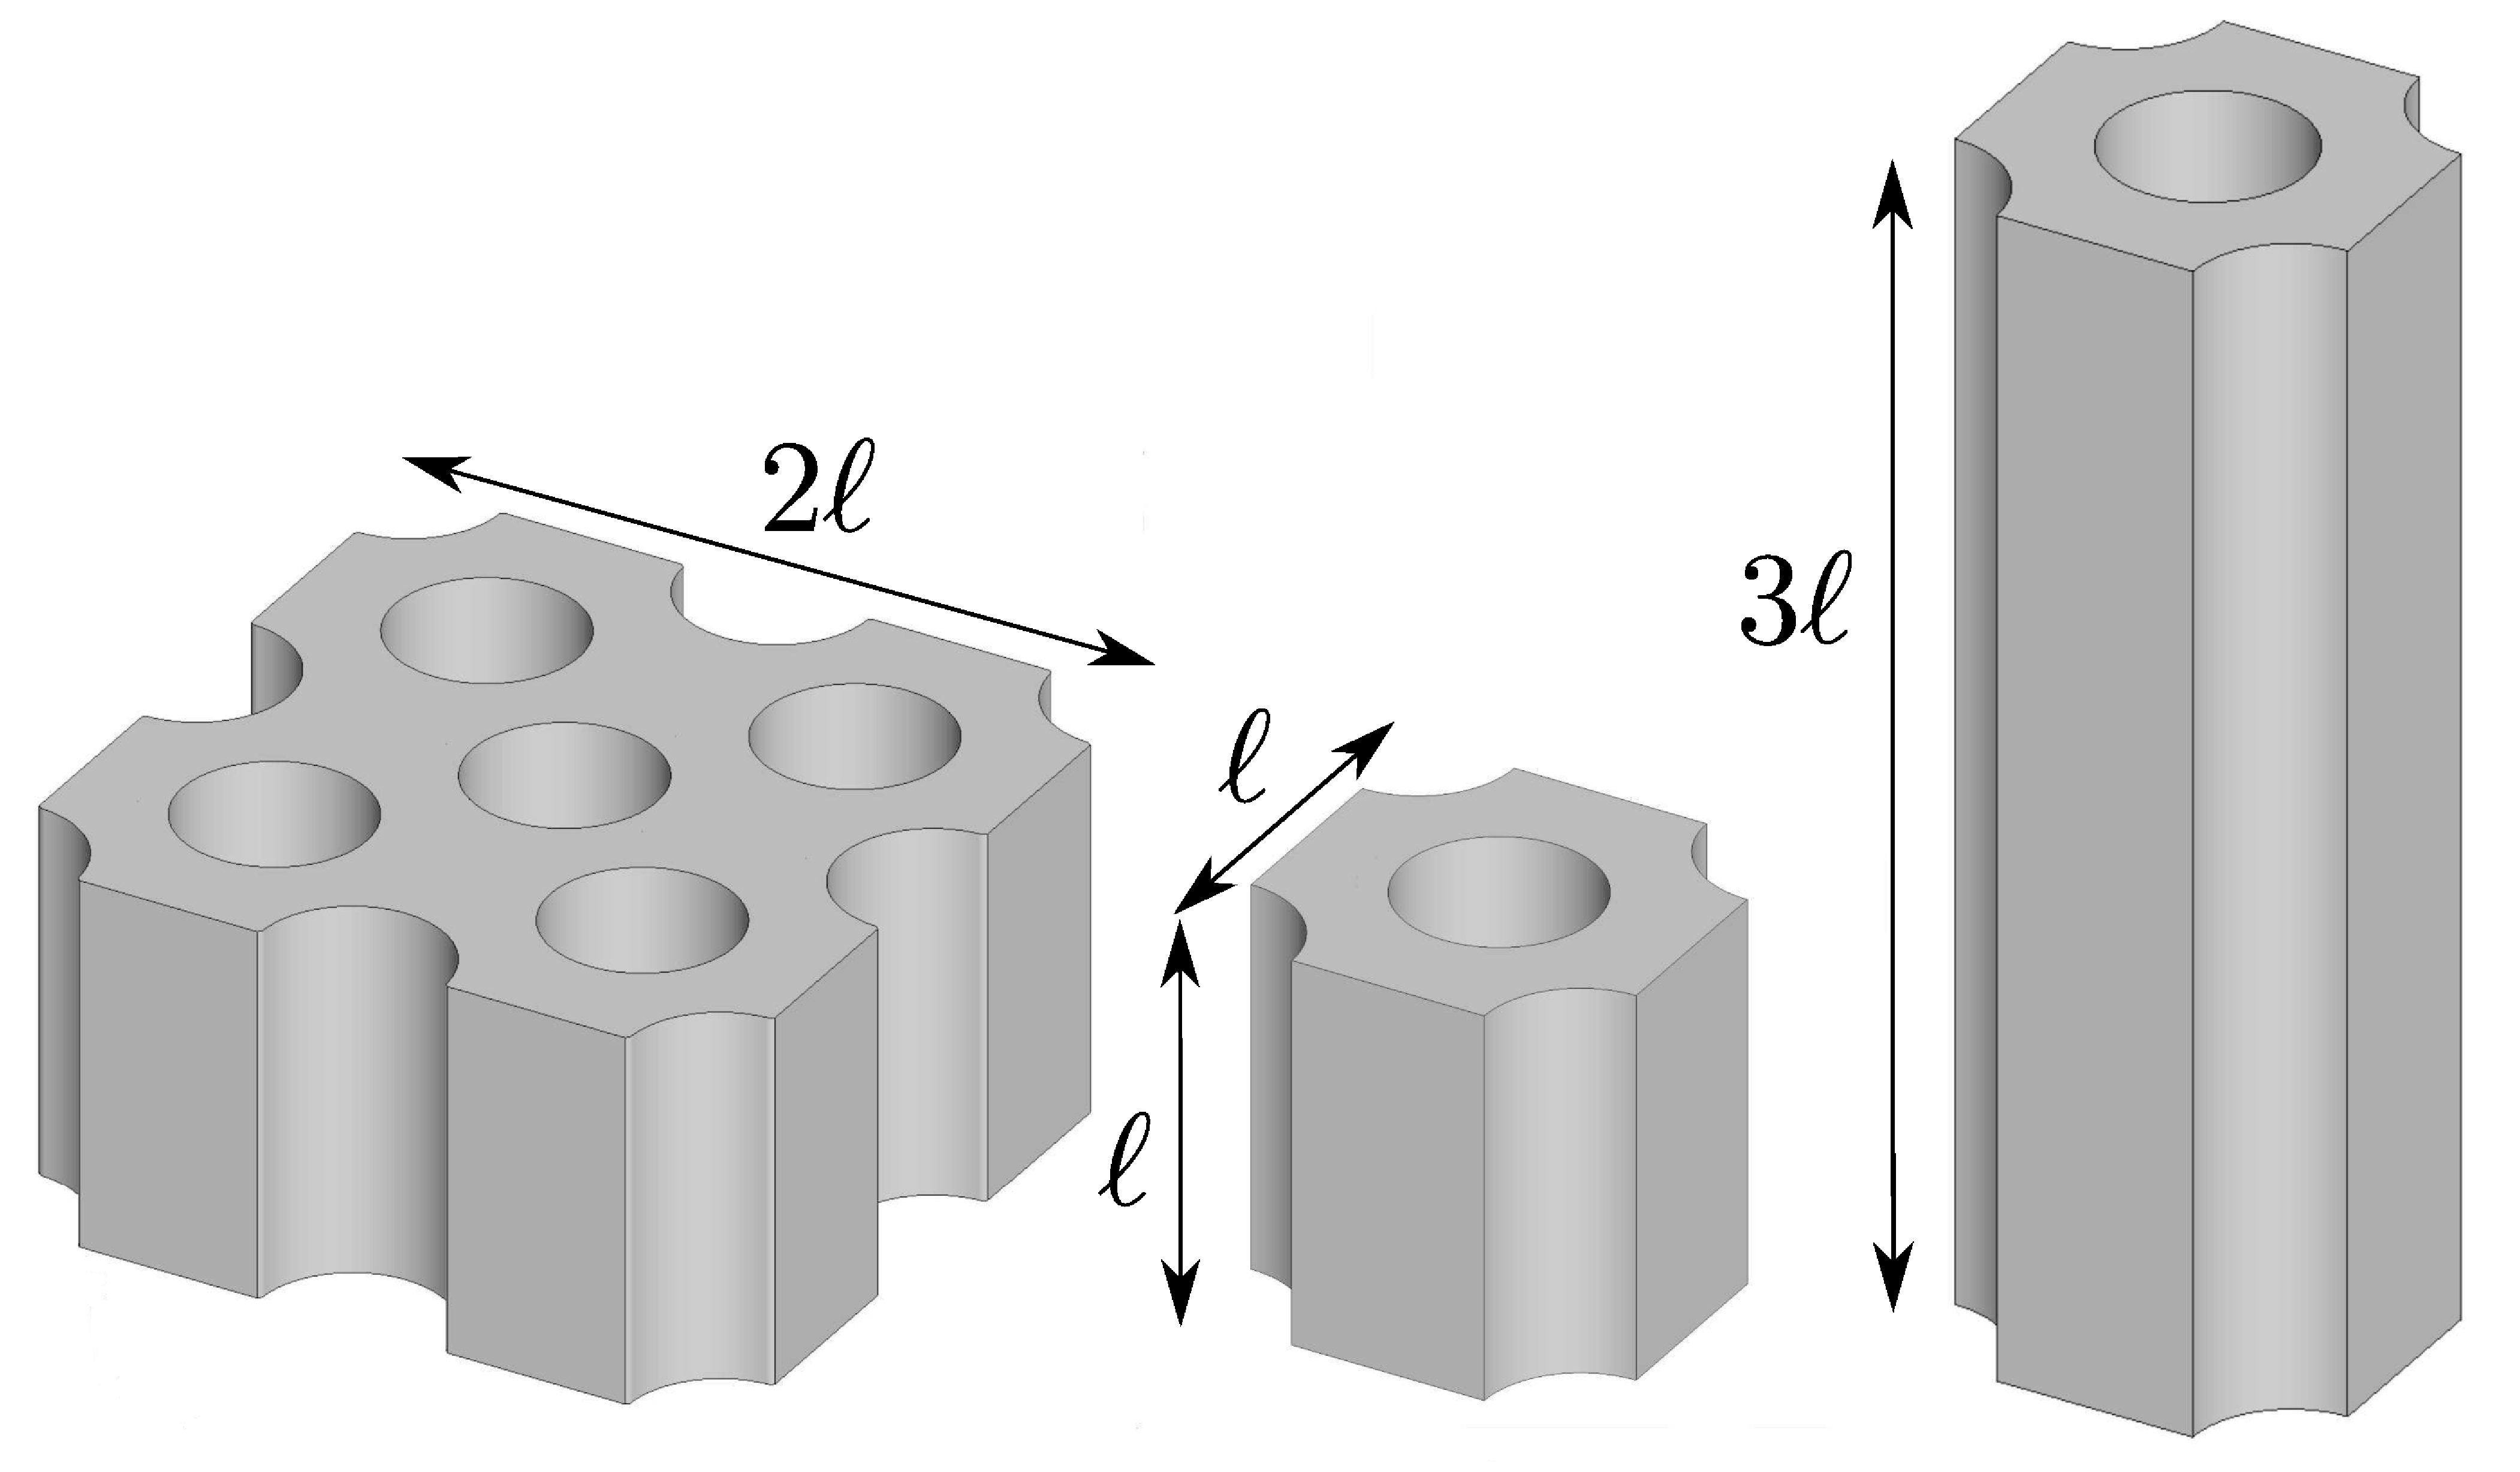
\includegraphics[width=0.8\textwidth]{chapter_4/figure/multiple}
	\caption{REV configurations. Left: $2 \times 2 \times 1$ arrangement; centre: $1 \times 1 \times 1$ arrangement (reference);  right $1 \times 1 \times 3$ arrangement.}
	\label{fig:multiple}
\end{figure}



%%%%%%%%%%%%%%%%%%%%%%%%%%%%%%%%%%%%%%%%%%%%%%%%%%%
\section{Microscopic solutions}
%%%%%%%%%%%%%%%%%%%%%%%%%%%%%%%%%%%%%%%%%%%%%%%%%%

In this section, some local microscopic fields computed with direct numerical simulations are shown, together with components of the intermediate tensor $\mathbf{M}$ coming from the numerical solution of the closure equations \eqref{eq:F_closure1}. 

In figure \ref{fig:1ch4} (top row) the local $x_1$ velocity component is drawn for the two-dimensional flow when $\varepsilon=0.6$, for three 
Reynolds numbers, to cover the transition from the Stokes to the inertial regime. In all plots, the velocities are rendered non-dimensional by
the corresponding value of 
$\displaystyle{\frac{K_{11}}{\nu_{\beta}} ||\bf{f}||}$. When inertia is absent, the flow has a central symmetry; by increasing the Reynolds number, only the 
symmetry with respect to the $x_1$ axis is maintained ($x_1$ is the direction of the forcing pressure gradient), with the wake's length which 
increases with $Re_d$. When $Re_d$ is of order 100 the wake spreads to the downstream boundary of the REV, re-entering, because of periodicity, 
at the upstream side.	This $Re_d$  represents the upper limit of validity for the cubic unit cell of side $\ell$; larger values of $Re_d$ 
could only be investigated with longer/larger/thicker REV's.

The non-dimensional local $M_{11}$ fields for the same parameters are displayed in figure \ref{fig:1ch4} (mid row). All values in the figures 
arise from scaling $\bf{M}$ with $\ell^2$. Visually, these local fields are strongly correlated to the local streamwise velocity component in the whole $Re_d$ range. 
This is not unexpected since the local velocity drives the convective term of system \eqref{eq:F_closure1}. 
The central symmetry of all components of $\bf{M}$ in the Stokes regime is coupled to the rotational invariance of the apparent permeability tensor in two-dimensional flows.

The effect of varying the porosity is shown in figure \ref{fig:1ch4} (bottom row) where $\varepsilon$ is taken equal to $0.4$. Even at such a
low porosity the stretching of the wake can be noticed, and it increases with $Re_d$. Interestingly, this effect is milder when
the forcing is inclined by an angle $\phi$, since the tighter packing of the inclusions causes a strong deviation of the mean flow along the axis of the fiber. In this case, $M_{11}$ and $M_ {22}$ behave very similarly to the case $\phi = 90^{\circ}$.    


\begin{figure}[H]
	\centering
	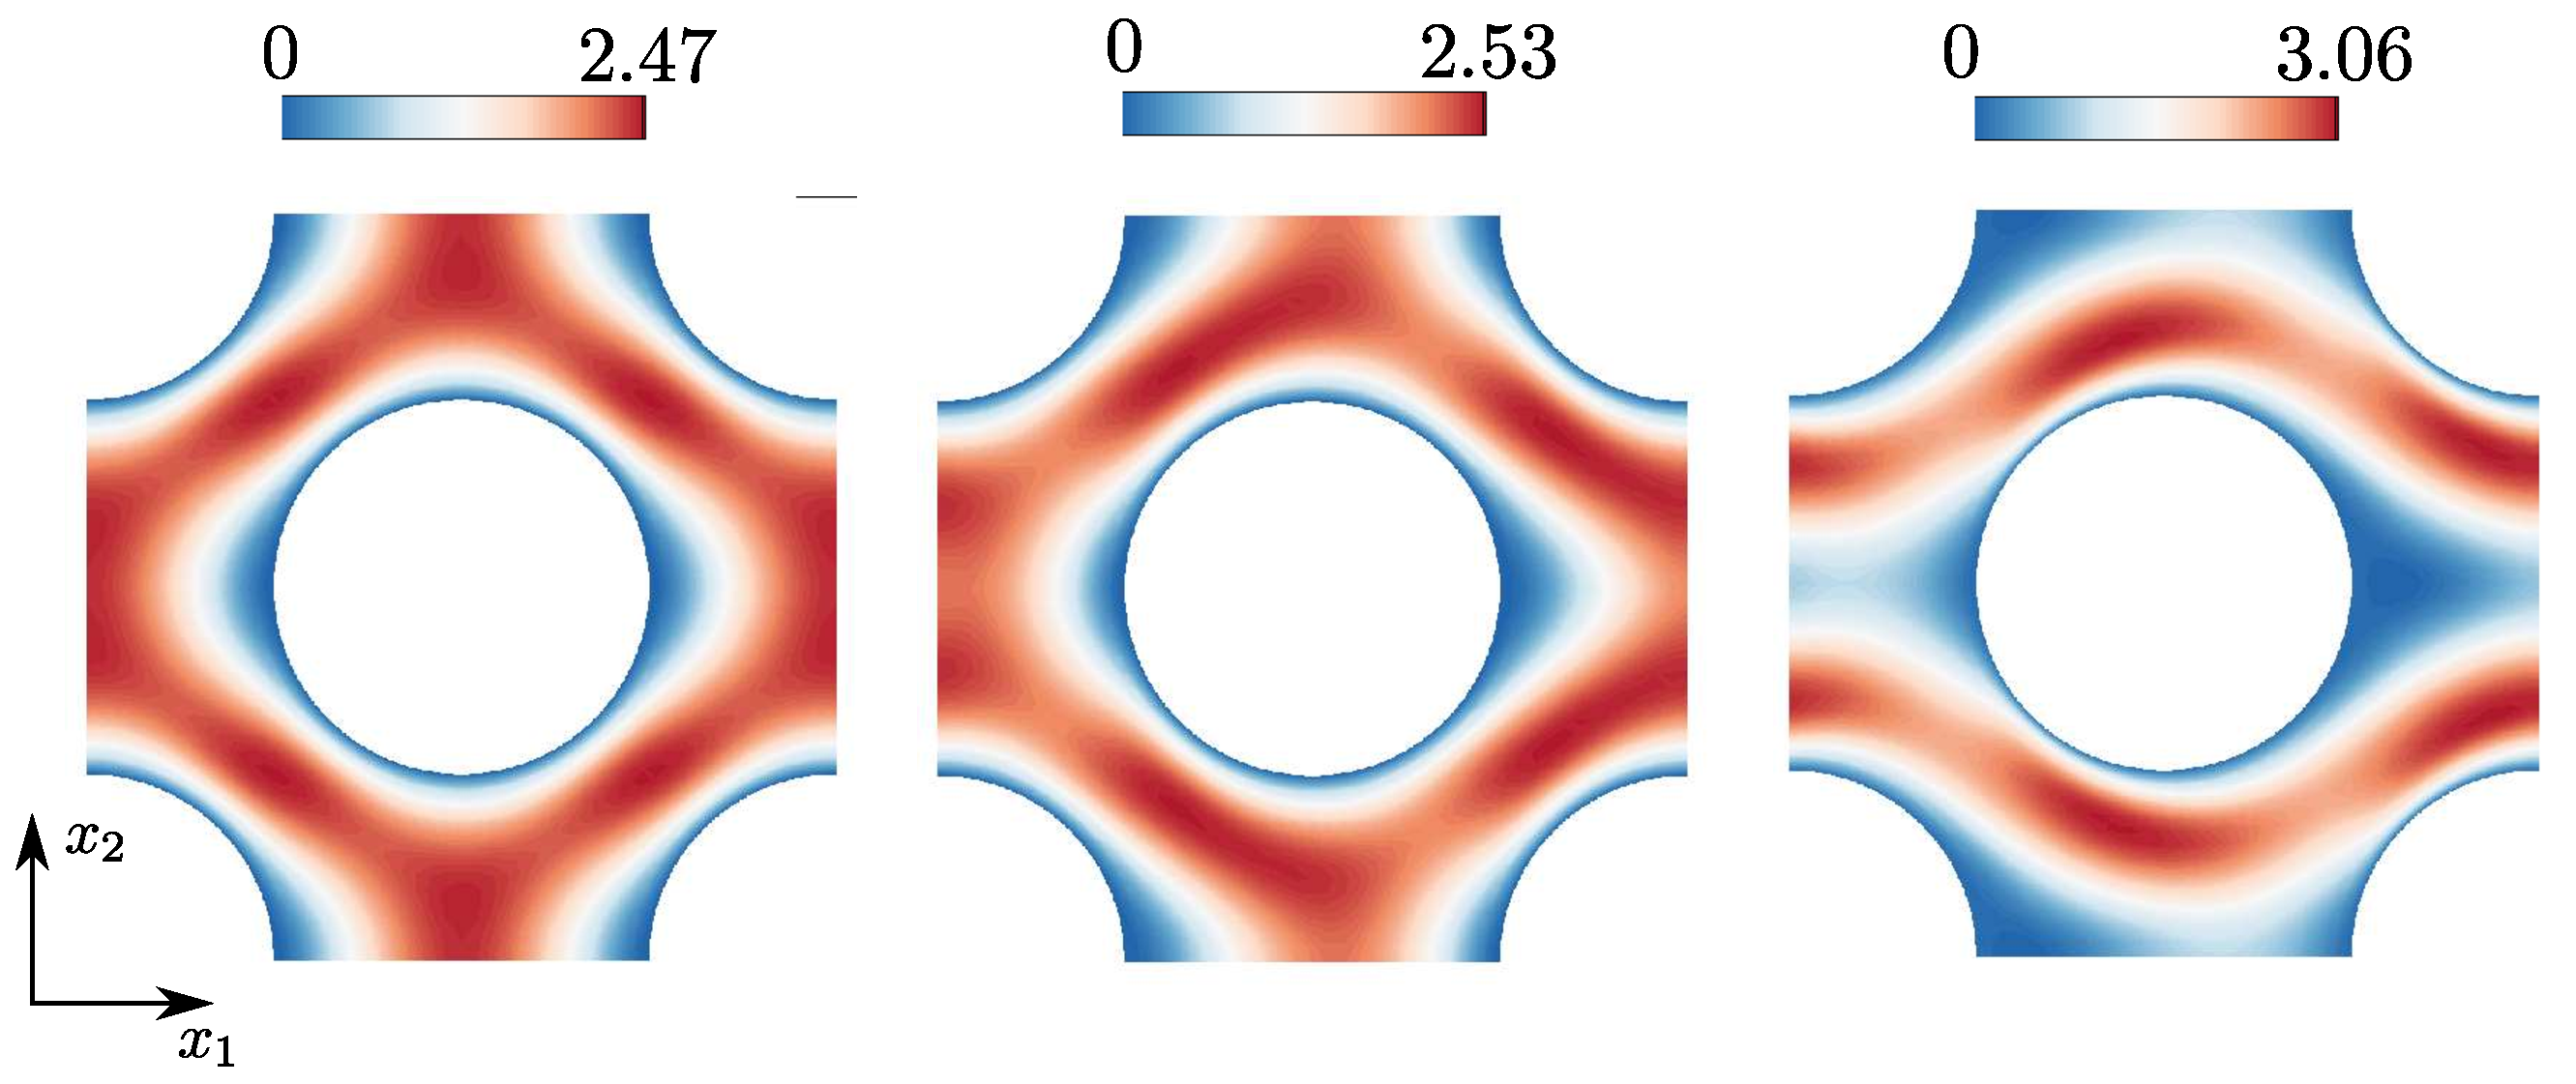
\includegraphics[width=1\textwidth]{chapter_4/figure/fig1}
	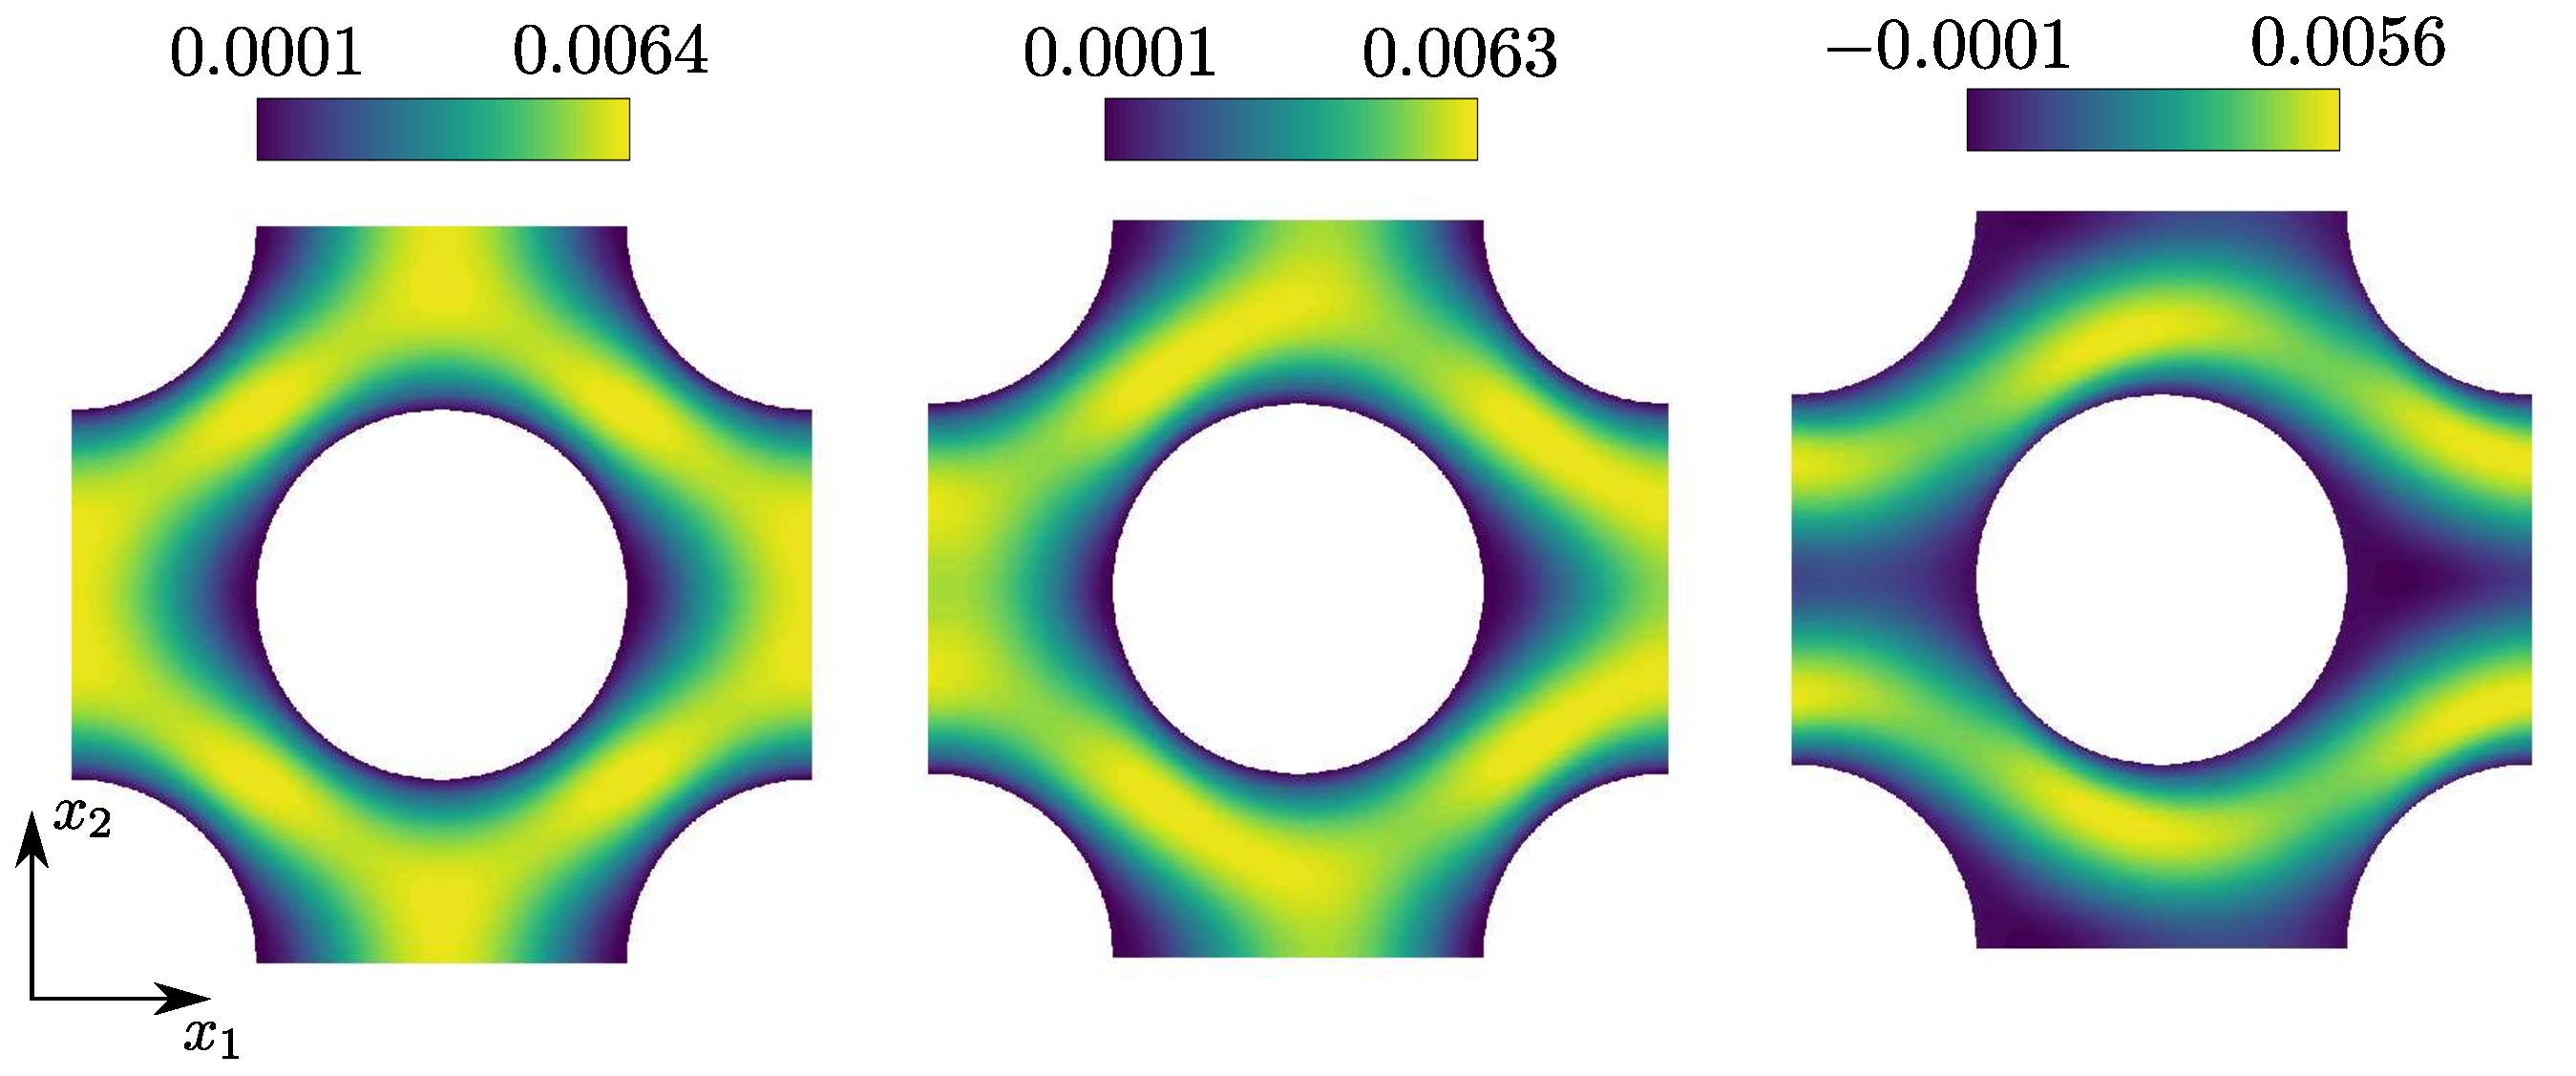
\includegraphics[width=1\textwidth]{chapter_4/figure/fig2}
	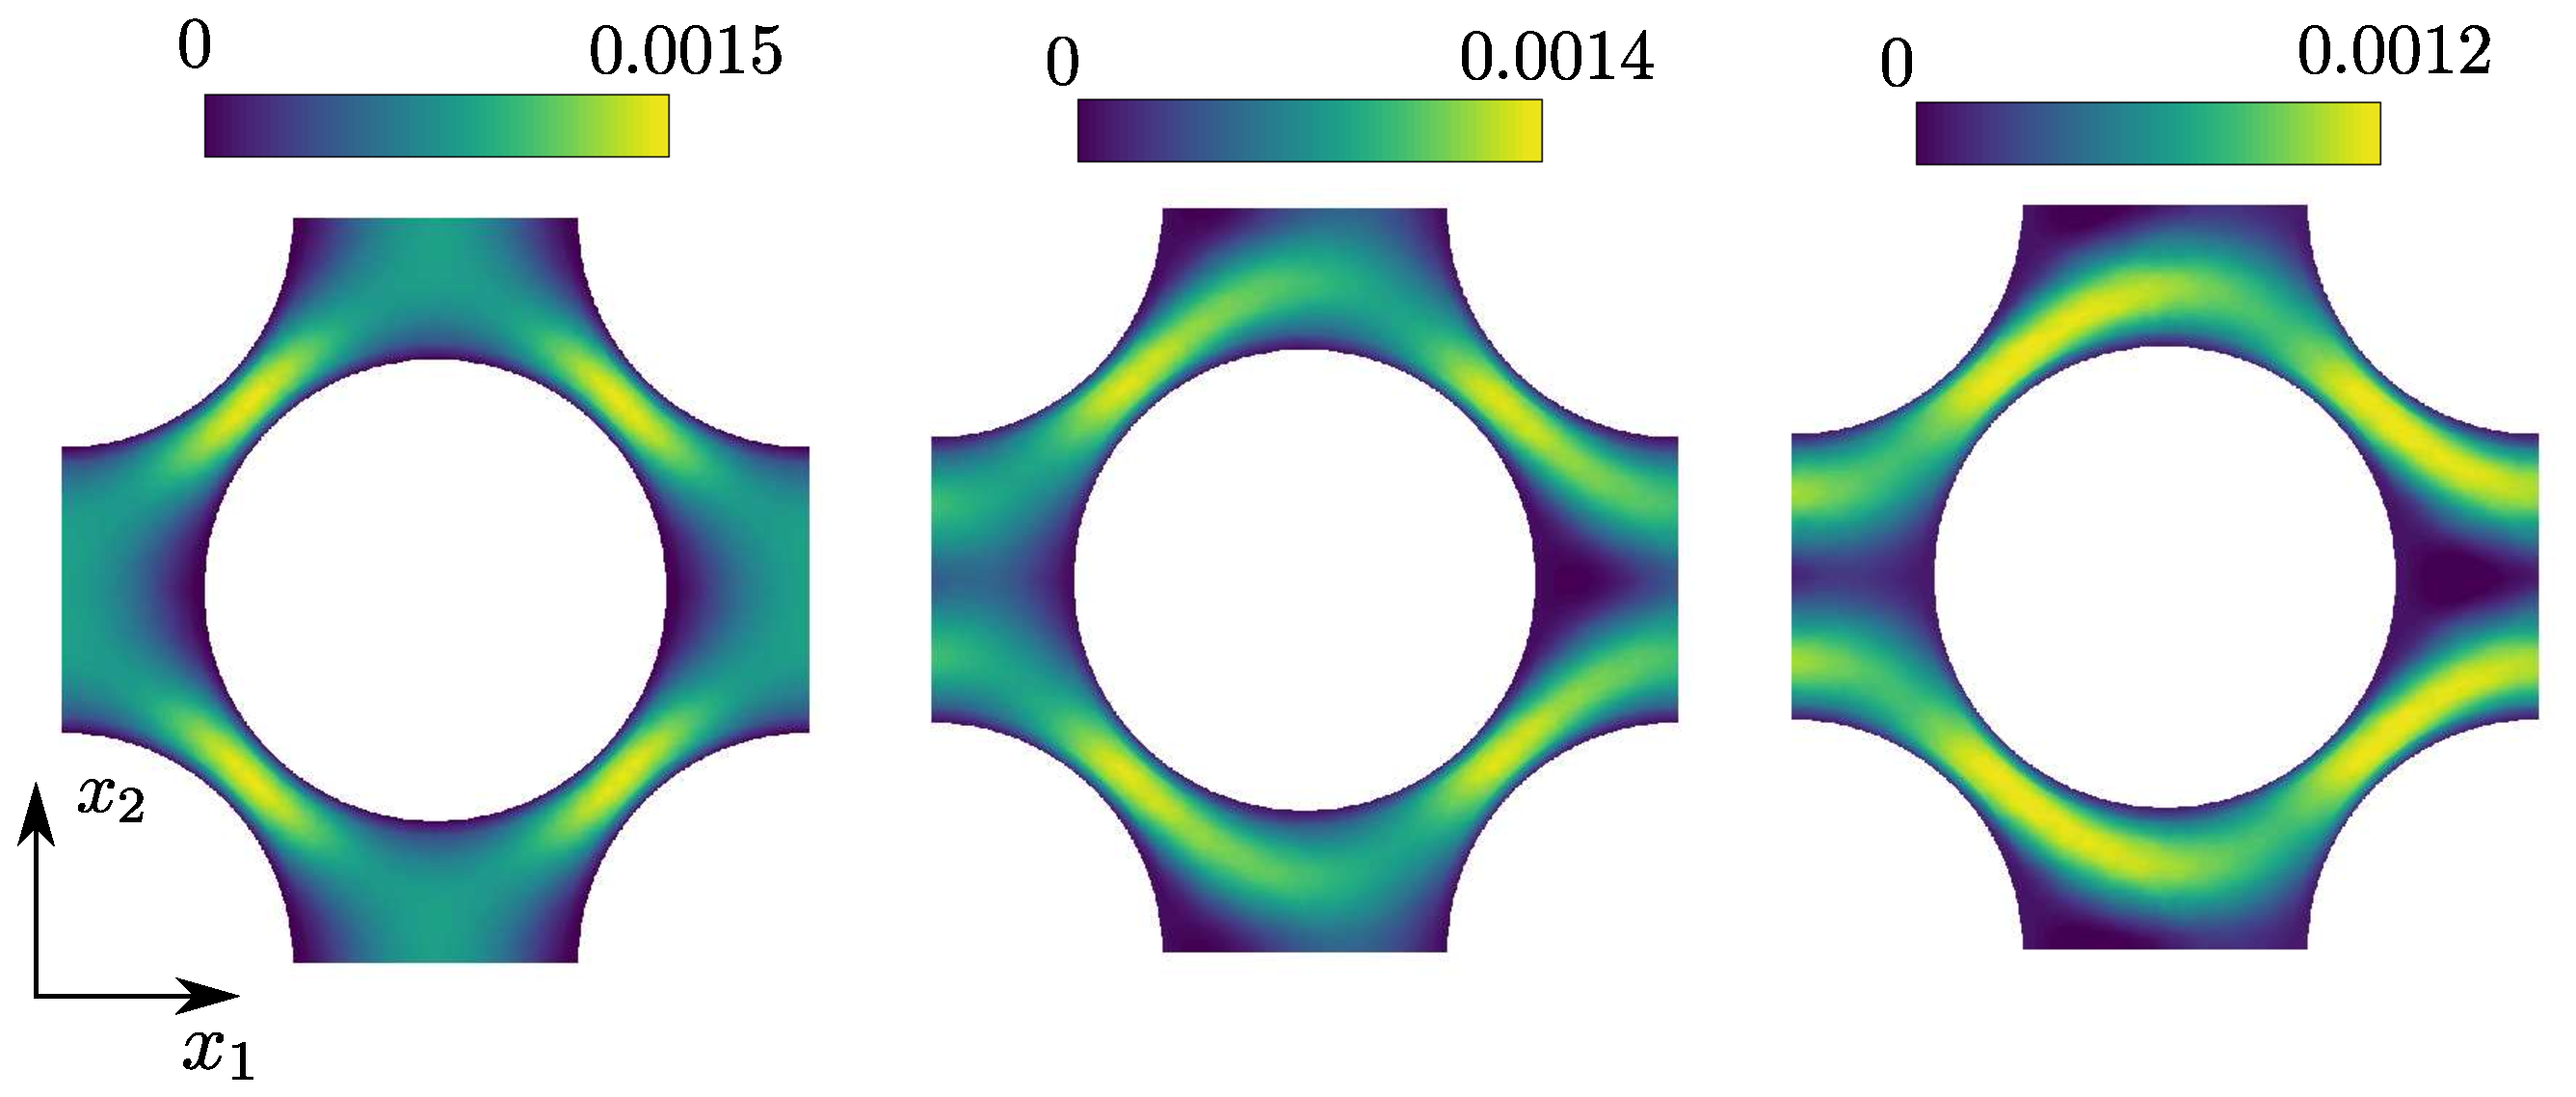
\includegraphics[width=1\textwidth]{chapter_4/figure/fig4}
	\caption{Top row: plane view of the dimensionless $x_1$ component of the local velocity field ${\vb}$ for the case $\theta=0,$ $\phi=0$, $\varepsilon=0.6$ and for three Reynolds numbers $Re_d$ = $0,10,50$, from left to right. Mid row: microscopic $M_{11}$ fields corresponding to the images in the top row. Bottom row: $M_{11}$ fields for the same Euler angles and Reynolds number as in the top two rows, and smaller porosity ($\varepsilon=0.4$).}
	\label{fig:1ch4}
\end{figure}


\newpage

Another interesting point emerges by inspection of  figure \ref{fig:3ch4} where two off-diagonal components of $\bf{M}$ are shown for two porosity 
values; the first image (left frame) represents a plane flow in the Stokes regime while the second is the plane cut of a three-dimensional 
solution in the inertial regime. Positive and negative values of the microscopic fields can be seen in both images but, once averaging is 
applied over the REV, the resulting permeability component is very close to zero (in fact, exactly equal to zero in the Stokes case).  This same features occurs for all off-diagonal terms in all cases examined, so that, within the current range of Reynolds numbers, the 
apparent permeability tensor is, to a good approximation, diagonal\footnote{In fact, there are always at least two orders of magnitude 
	differences between the diagonal and the off-diagonal components. While the latter should not, in principle, be ignored, we will focus attention 
	here only on the dominant terms of the permeability tensor.}.


\begin{figure}[H]
	\centering
	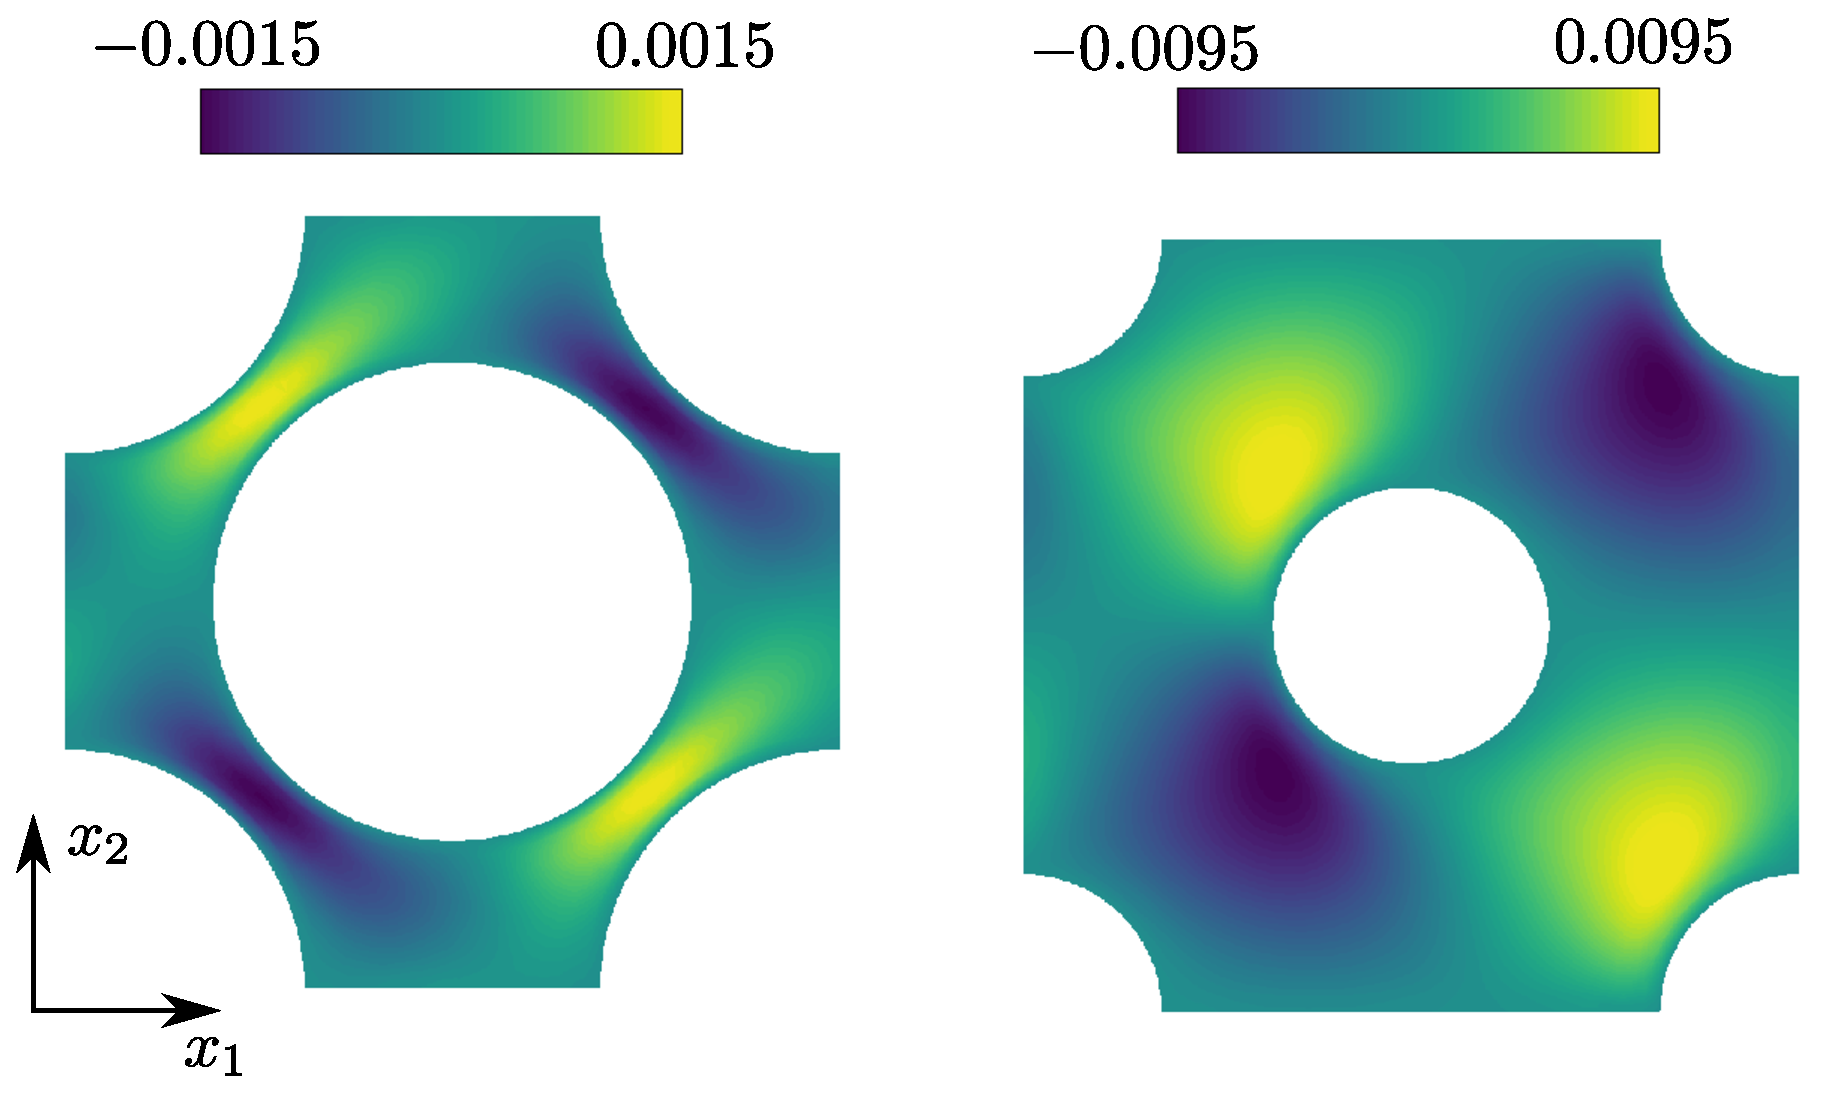
\includegraphics[width=0.8	\textwidth]{chapter_4/figure/fig3}
	\caption{right: Non-dimensional $M_{21}$ field for $\theta=0, \phi=0, Re_d=10, \varepsilon=0.8$, left: Non-dimensional $M_{12}$ field for $\theta=22.5^{\circ}, \phi=45^{\circ}, Re_d=50, \varepsilon=0.4$.}
	\label{fig:3ch4}
\end{figure}

A three-dimensional case is shown in  figure \ref{fig:5ch4}, where all the non-zero terms of the $\mathbf{M}$ tensor are plotted for a porous
structure with $\varepsilon=0.6$. The components shown are $M_{11}$, $M_{22}$,$M_{33}$, $M_{12}$ and $M_{21}$, while $M_{i3}$ and $M_{3j}$ are 
not plotted because they are identically zero to machine accuracy. Distinct features are visible in each image; in particular, in the last 
frame the $M_{33}$ microscopic component displays a low wavelength structure along the cylinder's axis. Increasing the dimensions of the REV 
along $x_3$ does not alter such a structure, i.e. the $\ell^3$ domain chosen with its periodic boundary conditions does not filter out 
significant high wave-numbers of the flow. We further note that the tensor $\mathbf{M}$ is not symmetric in this case since each off-diagonal component 
represents the solution of the closure problem in a specific direction (first index of the field) and the forcing term acts orthogonally to it
(second index of the field).  Once averaged over the REV it is found that both $H_{12}$ and $H_{21}$ are very close to zero.  


\begin{figure}[H]
	\centering
	\includegraphics[width=0.75\textwidth]{chapter_4/figure/fig5}
	\caption{Non-dimensional $\mathbf{M}$ components fields for the case $\theta=22.5^{\circ}, \phi=45^{\circ}, Re_d=50, \varepsilon=0.6$.}
	\label{fig:5ch4}
\end{figure}    






%%%%%%%%%%%%%%%%%%%%%%%%%%%%%%%%%%%%%%%%%%%%%%%%%%
\section{The apparent permeability tensor}
%%%%%%%%%%%%%%%%%%%%%%%%%%%%%%%%%%%%%%%%%%%%%%%%%%

\label{sec:5}

In this section the variations of the diagonal components of the permeability tensor $\mathbf{H}$ are discussed as function of the direction of 
the mean forcing, the Reynolds number and  the porosity. As stated previously, the Reynolds number ranges from $0$ to approximately $100$ in 
order to capture phenomena associated with inertia; the cases considered never lead to unsteady signals. 
The porosity parameter $\varepsilon$ is set to either $0.4$ (low porosity),  $0.6$ (medium) or
$0.8$ (high). The forcing direction is defined by the Euler angles and all the configurations considered in this section are summarized in 
table \ref{table:directions}; the choice has been made to explore a reasonably large range of parameters, with both two-dimensional and three-
dimensional flows characterized by symmetric and asymmetric patterns.

Let us briefly recall the methodology. First, a DNS is carried out to compute the microscopic flow. Then the  closure problem is solved for the 
tensor $\mathbf{M}$. Finally, each component of the apparent permeability  $\mathbf{H}$  is obtained by averaging (equation 
\eqref{eq:avg_intrinsic}).
The results are collected in figures \ref{fig:08_H}, \ref{fig:06_H} and \ref{fig:04_H}, showing the variation of the diagonal components 
of $\mathbf{H}$. 


\begin{table}[t]
	\centering
	\begin{tabular}{l | l l l}
		index & $\theta$ & $\phi$ & field properties \\\hline	\hline
		1 & $0^\circ$ & $0^\circ$ & 2D symmetric \\
		2 & $22.5^\circ$ & $0^\circ$ & 2D non-symmetric \\
		3 & $0^\circ$ & $45^\circ$ & 3D symmetric \\
		4 & $22.5^\circ$ & $45^\circ$ & 3D non-symmetric \\
		5 & $-$ & $90^\circ$ & 3D symmetric \\
		\hline  
	\end{tabular}
	\caption{Directions of the forcing tested and property of the solutions.}
	\label{table:directions}
\end{table}



\begin{figure}[H]
	\centering
	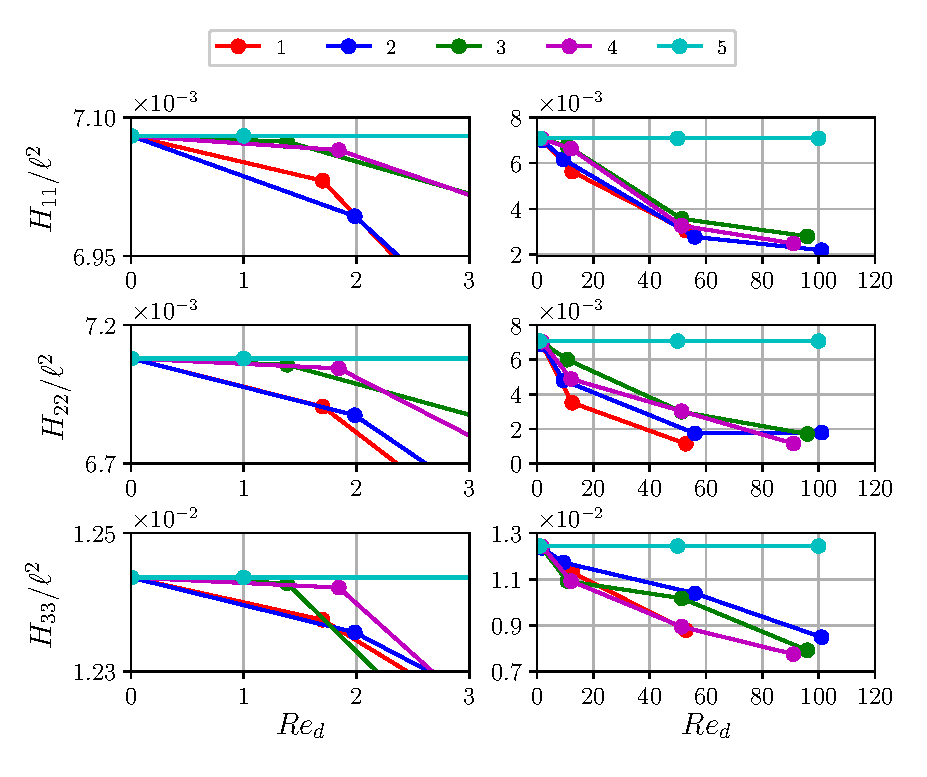
\includegraphics[width=1\textwidth]{chapter_4/figure/H_of08}
	\caption{Diagonal elements of the apparent permeability $\mathbf{H}$ as function of the Reynolds number for porosity  $\varepsilon=0.8$. The forcing  direction is represented through the couple of Euler  angles 
		$(\theta,\phi)$ (cf. table \ref{table:directions} for the case index). Left column: low-$Re_d$ regime; right column: inertial regime.}
	\label{fig:08_H}
\end{figure} 

\begin{figure}[H]
	\centering
	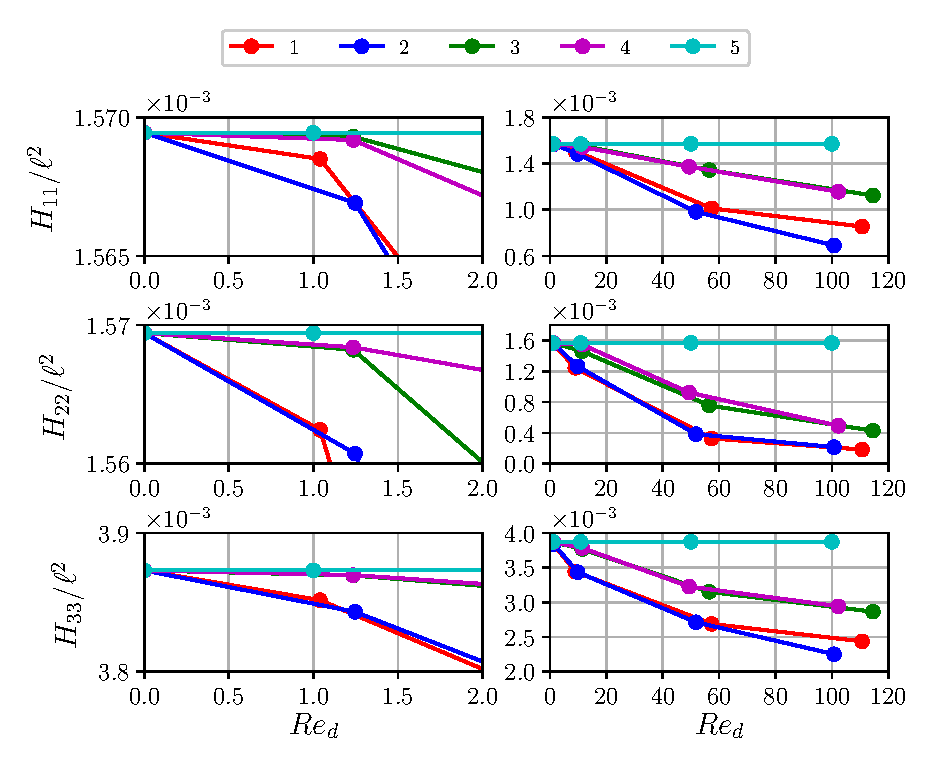
\includegraphics[width=1\textwidth]{chapter_4/figure/H_of06}
	\caption{Same as figure \ref{fig:08_H} with porosity $\varepsilon=0.6$.}
	\label{fig:06_H}
\end{figure}



\begin{figure}[H]
	\centering
	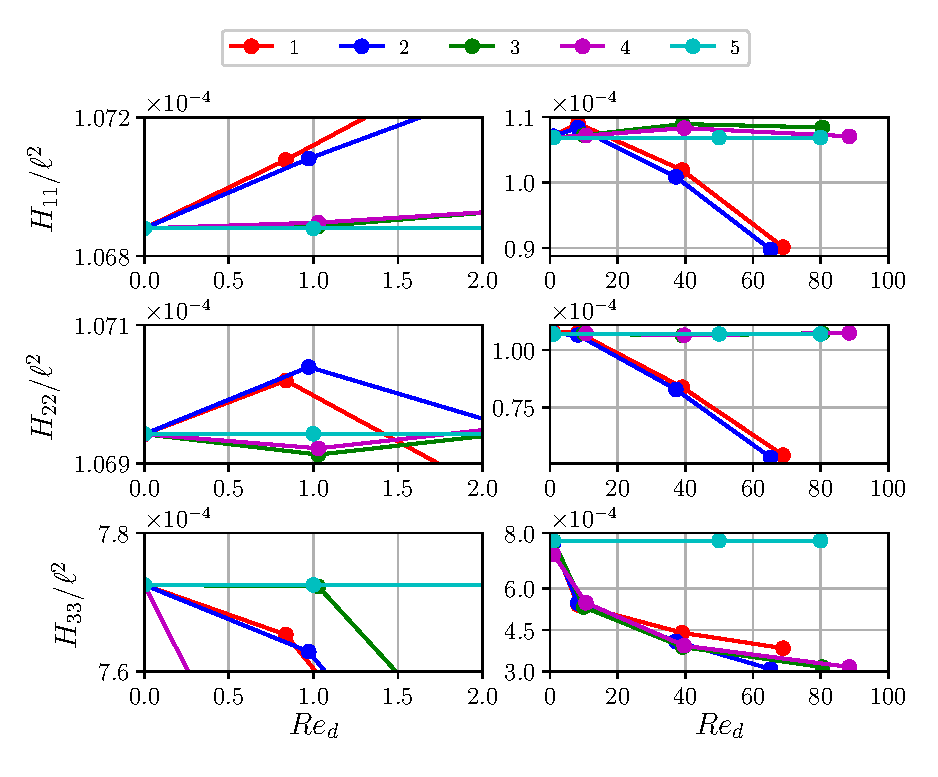
\includegraphics[width=1\textwidth]{chapter_4/figure/H_of04}
	\caption{Same as figure \ref{fig:08_H} with porosity $\varepsilon=0.4$.}
	\label{fig:04_H}
\end{figure}

%\begin{figure}[H]
%   \centering
%   \input{figure/H_of04.pdf_tex}
%   \caption{Same as figure \ref{fig:08_H} with porosity $\varepsilon=0.4$.}
%   %\label{fig:04_H}
%\end{figure}
%



In the left column of each figure we focus on the low-$Re_d$ regime ($0 < Re_d < 2$), while in the right column the effect of inertia can be 
assessed.  As expected, when $Re_d$ is small the apparent permeability is quasi-Reynolds-number-independent (and can be approximated well by 
the true permeability). As the Reynolds number increases above a few units, inertial effects grow in importance yielding typically a monotonic decrease of all 
components of $\mathbf{H}$, aside from case indexed 5 ($\phi=90^{\circ}$) for which the flow remains aligned with the cylinder's axis. In case 5 the 
microscopic flow solution is invariant with $x_3$ and does not change with $Re_d$ in the range considered, so that $\mathbf{H}$ is a  
constant tensor.

When the porosity is large all components show a similar behaviour irrespective of the forcing angle (except, clearly, case 5). Differences 
start appearing at $\varepsilon=0.6$; the two cases with $\phi=0^{\circ}$ (index 1 and 2) behave similarly, and so do the two cases indexed 3 
and 4 (with $\phi=45^{\circ}$). This seems to suggest a weaker effect of $\theta$ on the permeability components.  For even smaller porosity ($
\varepsilon=0.4$), the blockage which the inclusions cause to the flow produces the unexpected behaviour displayed in figure \ref{fig:04_H}. 
When the flow is purely two-dimensional (cases 1 and 2), variations in the Reynolds number affect $\mathbf{H}$ significantly; when a pressure 
gradient along $x_3$ is present the strong packing of the fibers constrain the fluid to flow prevalently along the fibers' axis, and the 
apparent permeability is almost $Re_d$-independent. When assessing variations in $H_{jj}$ for this case, attention should also be paid to the 
fact that the permeability is now at least one order of magnitude smaller than in the previous cases so that variations of the diagonal 
components shown in figure \ref{fig:04_H} are tiny in absolute terms.  This is related to the fact that  the  inverse of the permeability  
plays the role of a drag coefficient in the macroscopic expression of the force  (cf. equation \eqref{eq:macroscale}).  In other words, 
materials with higher porosity (larger space between solid inclusions) offer lower resistance to the motion of the fluid.


%In the simulations carried out the off-diagonal terms are consistently at least two orders of magnitude smaller than their diagonal 
%counterparts, for all parameters considered.  
Applying the intrinsic average operator to the non-diagonal component of the tensor $\mathbf{M}$ results in terms that are negligible with respect to their diagonal counterparts, and these results are true for all the parameters considered. This means that there is a very weak coupling between the principal directions of the fiber.
The directional decoupling and the diagonal property of the apparent permeability tensor has also been computationally demonstrated
on a completely different REV geometry by \citet{soulaine2014}. Conversely,
\citet{lasseux} have carried out a two-dimensional study with fibers of square cross-section, finding that the off-diagonal terms are 
non-negligible and only about
one order of magnitude smaller than the diagonal components. This result is a consequence of the non-rotationally-invariant  geometry  
considered.  The present work and the two articles just cited suggest that the  diagonal property of the tensor $\mathbf{H}$   is closely
related to the geometry of the porous material, more  than to the flow regime.  



%%%%%%%%%%%%%%%%%%%%%%%%%%%%%%%%%%%%%%%%%%%%%%%%%%%%%%%%%%%
\section{A metamodel for $\bf H$}
%%%%%%%%%%%%%%%%%%%%%%%%%%%%%%%%%%%%%%%%%%%%%%%%%%%%%%%%%%%

The previous sections has shown how the apparent permeability depends on  the two Euler angles, the Reynolds number and the porosity. The space 
of parameters is formidable and the results found so far are not sufficient to treat, for example, cases characterized by multiple inclusions'
sizes and orientations in different regions of the domain, or cases involving a poroelastic medium, with temporally and spatially varying 
porosity, flow direction and local Reynolds number. The complete solution of the closure problem for a single set of parameters takes 
approximately 4 CPU hours on our two-processor Intel(r) IVYBRIDGE 2.8Ghz, each with 10 cores and 64 GB of RAM, so that a complete parametric 
study is, to say the least, unpractical. In view of this, the construction of a metamodel capable to provide a full characterisation of the 
permeability as a function of all parameters is a worthy endeavor. We have tested several surrogate models, before eventually settling on the kriging 
approach \cite{Kleijnen20171} described in the following.



%Usually the homogenization approaches are used to investigate complex problems in which   length scales  of the physical phenomena are much %larger than the REV one (\citet{ugis})  (\citet{prosperetti}). The aim
%is to avoid to resolve the  length scales smaller the unity (with respect to the REV length) and in consequence to drastically reduce  the %number of mesh cells and the computational load.
%Here the physics at the REV scale is modelled with the VANS method and in particular by identifying the local apparent permeability $%\mathbf{H}$ tensor.

%In addition, it has been shown that the non constant tensor $\mathbf{H}$ required to be evaluated locally and at each time step  in a full %temporal simulation over a large domain with large REV numbers. 
%Especially, at at least the local Reynolds number and the flow direction change from cell to cell, where each cell could be composed of one or %several REV.

%Solving the $\mathbf{H}$ closure problem for a given set of parameters takes approximately 4 hours with our resources [two processor Intel(r) %IVYBRIDGE 2,8Ghz each with 10 cores and 64 GB of RAM], so reiterate the procedure inside each time step for each cell is at least unpractical. 
%
%To circumvent such a problem  the design of a reduce order model, or the use of a metal-model can be a convenient approach.  
%In this work, several metamodel have been investigated and only one is presented in the following.


%%%%%%%%%%%%%%%%%%%%%%%%%%%%%%%%%%%%%%%%%%%%%%%%%%%%%%%%%%%
\subsection{DACE sampling}
%%%%%%%%%%%%%%%%%%%%%%%%%%%%%%%%%%%%%%%%%%%%%%%%%%%%%%%%%%%


The first step to build a metamodel is the collection of relevant samples.
The quality of the final metamodel strongly depends on the samples collected and their number and distribution is of primary importance.
The apparent permeability tensor, $\mathbf{H}$, depends on  four independent variables; the samples  have been generated starting from 
the set of parameters given in table \ref{table:DACE}.

\begin{table}[t]
	\centering
	\begin{tabular}{l | l l l l l}
		parameter & values \hs{0.5} & \hs{1.5}       &  \hs{1.5}     &\hs{1.5}   &\hs{1.5}  \\ \hline \hline
		$\theta$  & $0^\circ$     & $22.5^\circ$ & $45^\circ$  &  & \\
		$\phi$    & $0^\circ$     & $22.5^\circ$ & $45^\circ$  & $67.5^{\circ}$ & $90^{\circ}$ \\
		$Re_d$ & $0$ & $10$ & $50$ & $100$ \\
		$\varepsilon$ & $0.4$ & $0.6$ & $0.8$ \\
		\hline  
	\end{tabular}
	\caption{Sampling parameters.}
	\label{table:DACE}
	
\end{table}

One of the best options to generate the relevant database would be to use a full factorial design approach
in which all the combinations of the four variables from table \ref{table:DACE} are computed. Because of the large number of computations required, this approach has not been retained. We have resorted to the methodology known as DACE (Design and Analysis of
Computer Experiments), a technique to fill in the best possible way the space of the parameters of the problem.
%
%Actually, to be more efficient, we have to use the methodologies developed for the design and analysis of computer experiment refers as DACE. %DACE models 
%are canonical methods that fills in the best way the space parameters of the problem, knowing  the number of variables and their discrete %values. 
The Dakota library \cite{dakota} has been selected for the purpose and 
the Monte-Carlo incremental random sampling algorithm \cite{giunta} has been chosen, in order to make efficient use of the cases
already computed. This incremental approach selects in a quasi-random way the new samples to generate, starting from the existing ones. In the end, the set of samples comprises 118 cases.


% to keep the advantage of the previous simulations and to decrease the number of new cases to carry out.
%Stating from the previous samples already computed, 30 new sampling have been generated by the algorithm that fill the parameters space in a %quasi-random way. 
%Each new sampling parameters depends on the previous set.
%
%For each new parameters combination we repeating the computational procedure explained before to compute the permeability tensor  $\mathbf{H}$.



\begin{figure}[H]
	\centering
	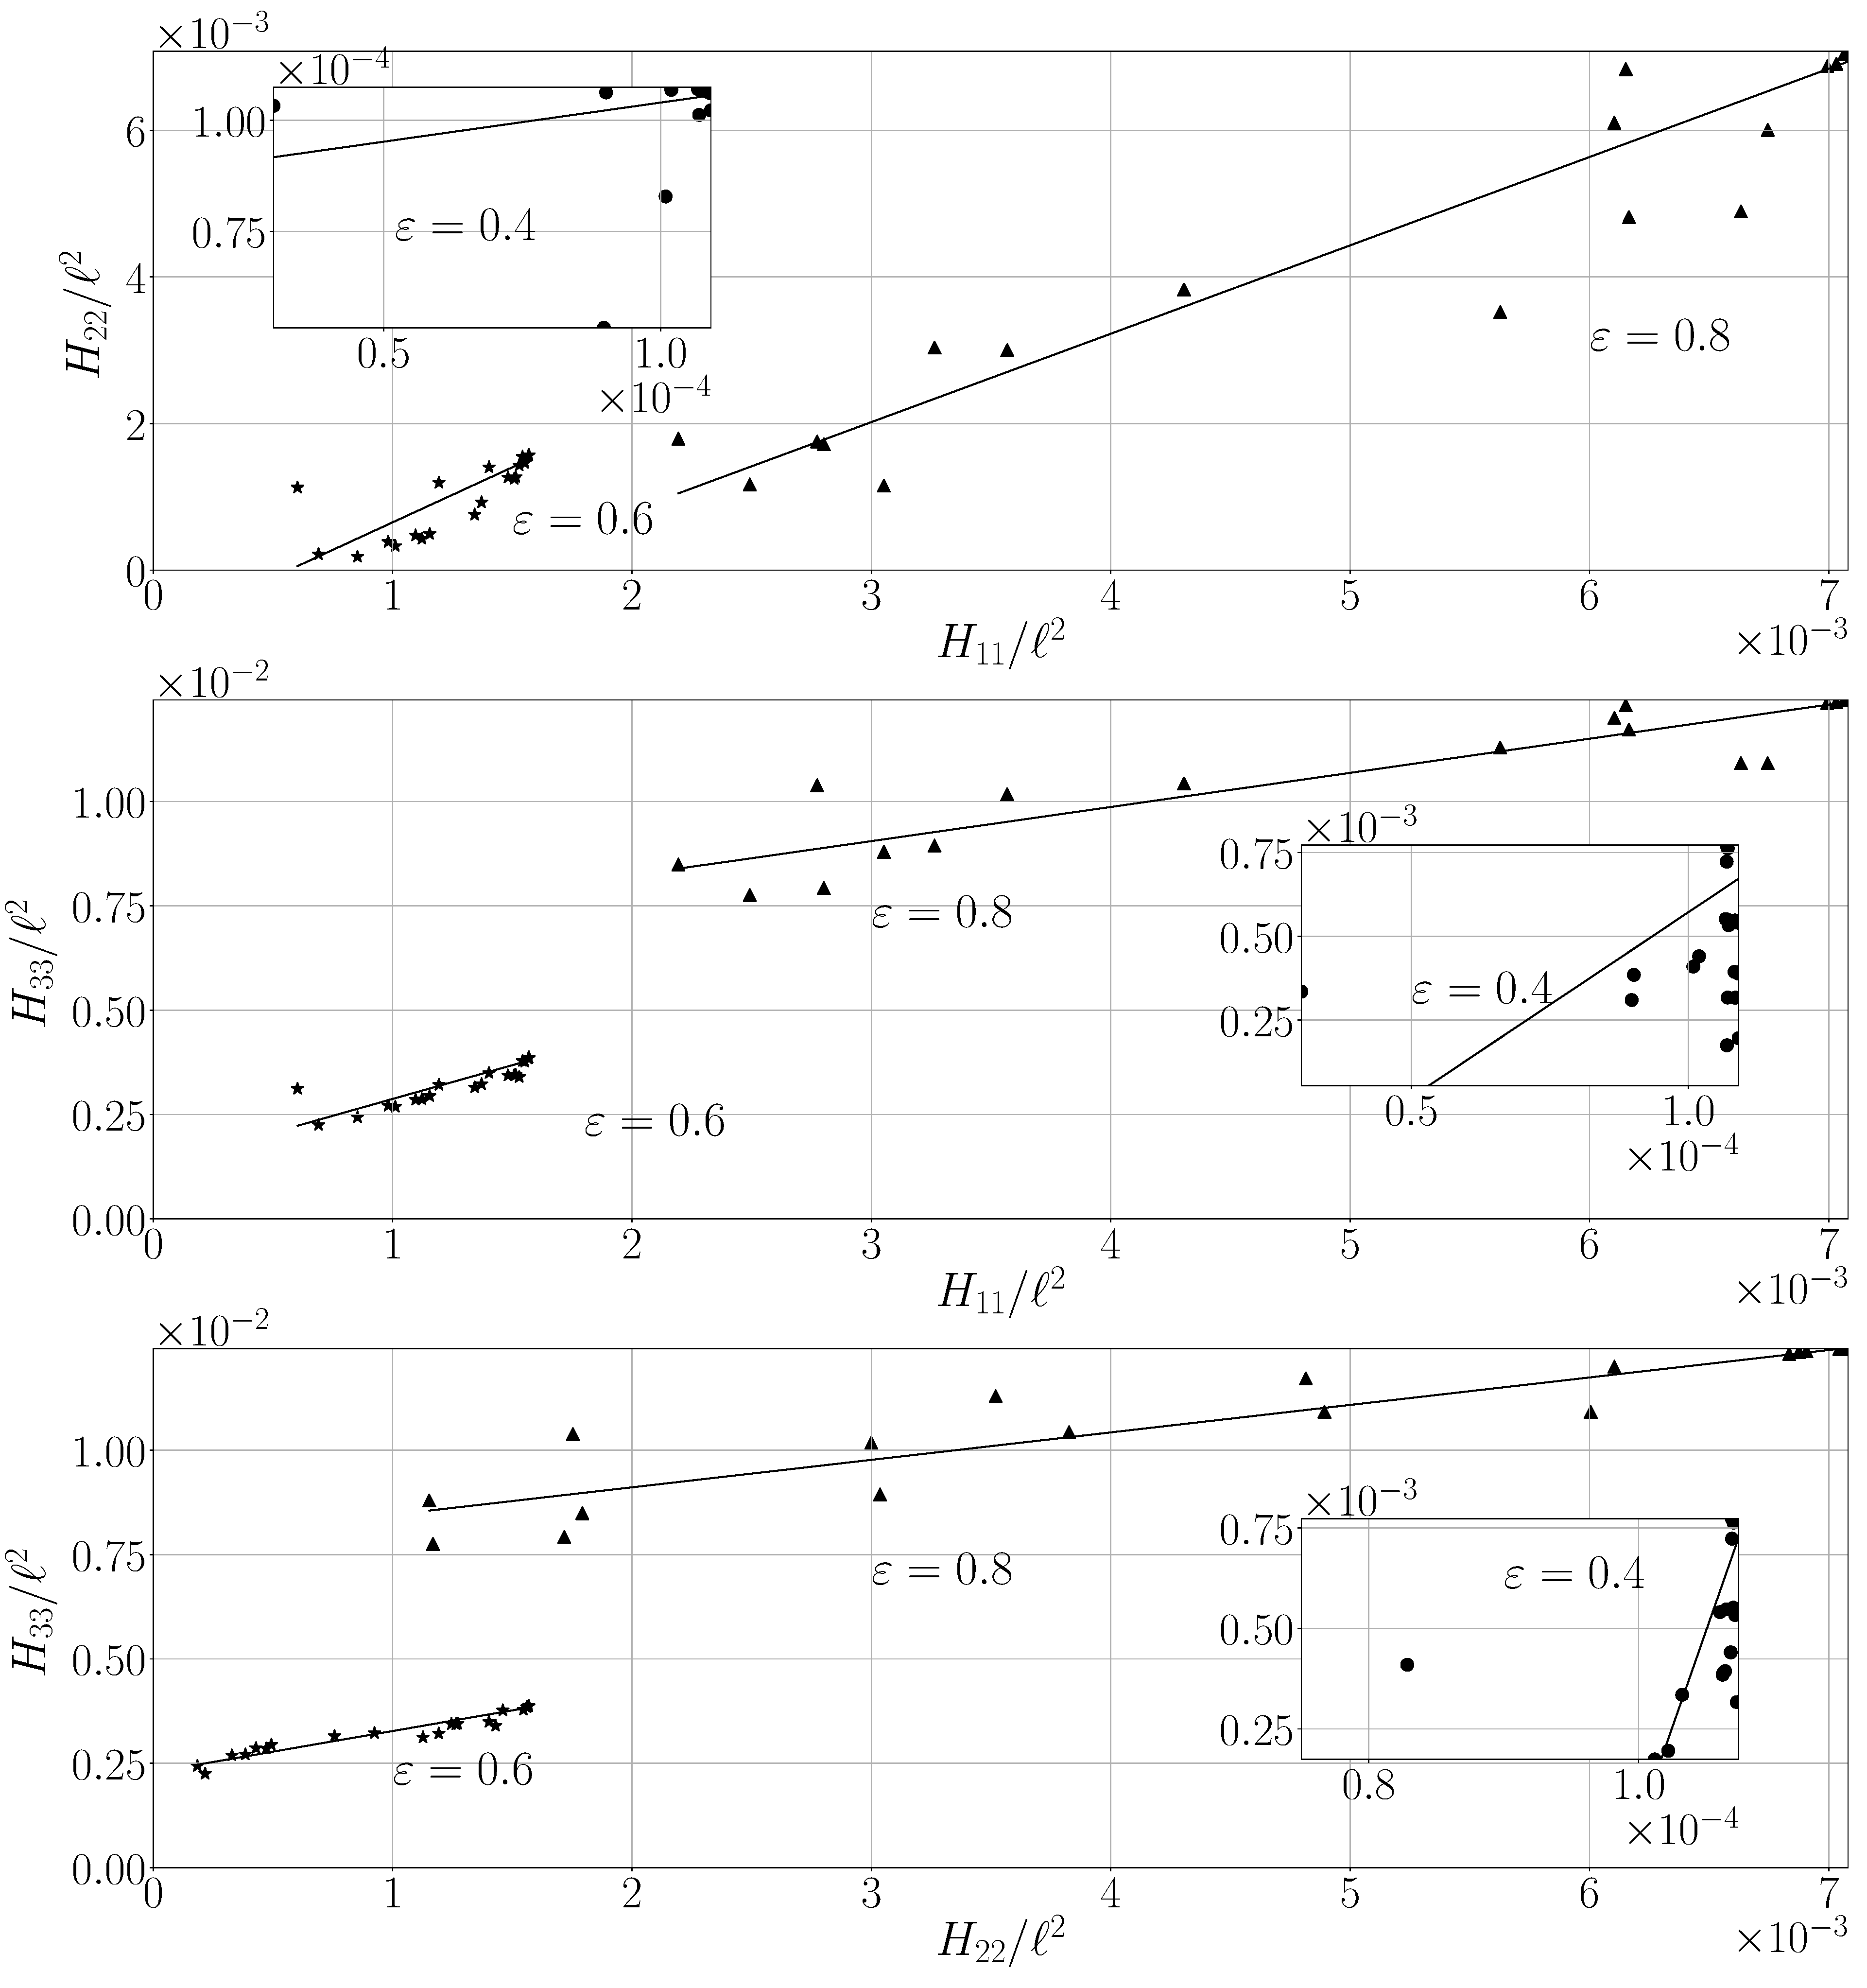
\includegraphics[width=1\linewidth]{chapter_4/figure/scatter_matrix}
	\caption{Scatter matrix plot for the collected numerical data of the apparent permeability tensor.}
	\label{fig:scatter_matrix}
\end{figure}



In the scatter plot of figure \ref{fig:scatter_matrix} the three diagonal components of the permeability tensor are shown 
as function of one another. The three porosities are separately considered in each of the above plot, and the permeability points are 
represented with their linear regression on top. This kind of plot is common in statistical analysis to determine if correlations in the data 
are present.  The permeability components show some correlation with the data points which lie reasonably well on a straight line. This
result has a physical implication.
Remembering the diagonal dominance of the permeability tensor, we have in the low
$Re_d$ limit: 

\begin{equation}
\left( \meani{u_{\beta}},\meani{v_{\beta}} , \meani{w_{\beta}}\right) \sim \left(H_{11} \dfrac{{\partial p}}{\partial x_1}, H_{22} \dfrac{{\partial p}}{\partial x_2} ,  H_{33} \dfrac{{\partial p}}{\partial x_3}\right).
\label{eq:linear_k}
\end{equation}
$$ \, $$
\noindent It is then possible to compute the angle between the forcing term, $\nabla p$, and the average velocity vector, represented 
in  figure \ref{fig:diag_rel} for the two-dimensional case, $\phi = 0$. This is achieved by taking the ratio between the
first two components of Darcy's equation, calling $\gamma$ the flow deviation with respect to the mean forcing. We thus have:

\begin{equation}
\tan \, (\theta + \gamma) = \dfrac{H_{22}}{H_{11}} \tan \, \theta.
\label{eq:angles}
\end{equation}

\noindent If the ratio between the two permeability components is equal to one, the angle $\gamma$ vanishes.
The correlation between $H_{11}$ and $H_{22}$ controls the deviation of the flow in the $(x_1, x_2)$ plane, and the argument
can easily be extended to $H_{11}/H_{33}$ and $H_{22}/H_{33}$  for deviation angles in three-dimensions.

\begin{figure}[H]
	\centering
	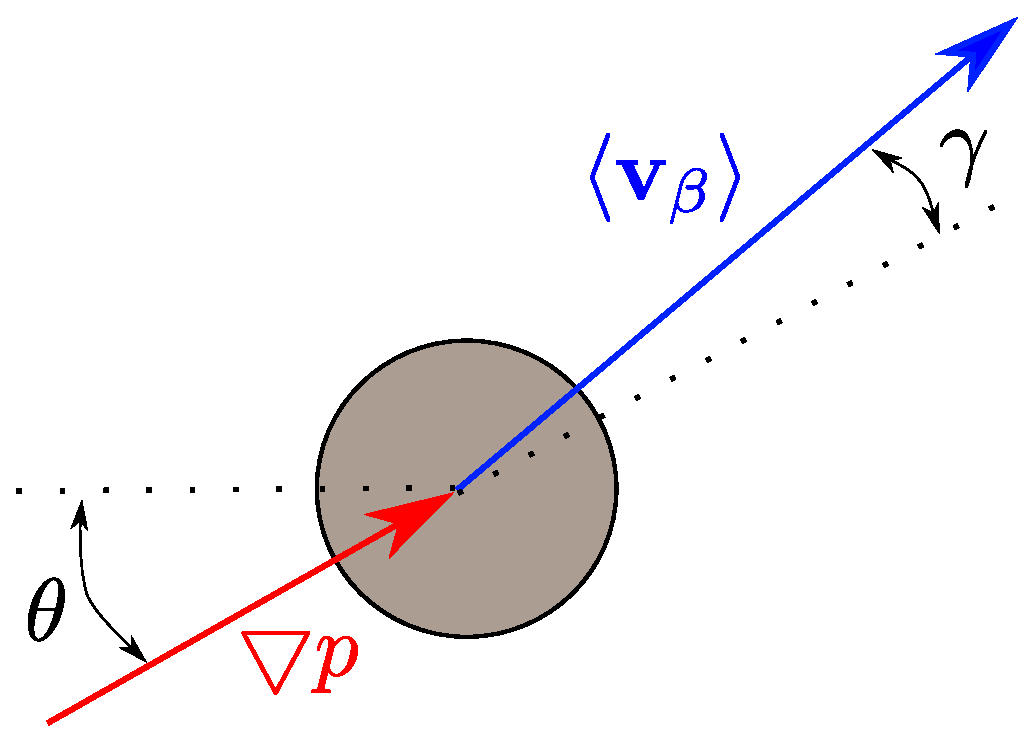
\includegraphics[width=0.45\linewidth]{chapter_4/figure/k11_k22_relation}
	\caption{Explanatory sketch for the relation between mean pressure gradient and mean velocity field.}
	\label{fig:diag_rel}
\end{figure}


\begin{table}[t]
	\centering
	\begin{tabular}{ l | l   l   l   }
		$\varepsilon$ & $H_{11}/H_{22}$ \hs{1} & $H_{11}/H_{33}$ \hs{1} & $H_{22}/H_{33}$ \hs{1} \\ \hline \hline
		0.4 & 1.57 & 11.06 & 96.03 \\ 
		0.6 & 1.50 & 1.62 & 0.99 \\
		0.8 & 1.20  & 0.82 & 0.66 \\ \hline
	\end{tabular}
	\caption{Permeability components ratio for three values of the porosity. The permeability ratios here are given by the angular coefficients of the linear correlations displayed in figure \ref{fig:scatter_matrix}.}
	\label{table:ratio}
\end{table}

Using a linear correlation such as that shown in table \ref{table:ratio} and  figure \ref{fig:scatter_matrix}, it is 
observed that in the low porosity case $(\varepsilon=0.4)$ the ratio can become very large indicating a strong deviation of the flow from the forcing direction, because of the strong constraint provided by the inclusions. As the porosity increases, the ratio does not differ much from unity, which means that the deviation remains limited. It is simple to see that
the deviation angle, for example in the $(x_1, x_2)$ plane, satisfies the approximate relation
$$
\tan \, \gamma = \dfrac{\left(1 - \dfrac{H_{11}}{H_{22}}\right) \tan \, \theta}{\dfrac{H_{11}}{H_{22}} + \tan^2 \, \theta},
$$
so that for $\dfrac{H_{11}}{H_{22}}$ equal to, say, 1.5, the largest deviation remains always below $12^{\circ}$ for any $\theta$.
It should however be kept in mind that trends based on these ratios are valid only as long as Darcy's law and linear correlations
are acceptable. Cases exists for which such trends are violated; for example, a flow with $\theta = 45^{\circ}$ and $\phi = 0^{\circ}$ has
deviation angle $\gamma$ equal to zero, for whatever porosity. In this case $H_{11}/H_{22}$ is equal to one and such a point is an 
outlier in the regression plots of figure \ref{fig:scatter_matrix}.


%%%%%%%%%%%%%%%%%%%%%%%%%%%%%%%%%%%%%%%%%%%%
\subsection{Kriging interpolation method}
%%%%%%%%%%%%%%%%%%%%%%%%%%%%%%%%%%%%%%%%%%%%

The kriging approach is a linear interpolation/extrapolation method that aims to build a predictor field
based on a set of observations  $(\mathbf{x_i}, y(\mathbf{x_i}))$,  for $i=1,...,n$. 

The predictor $\hat{f}(\mathbf{x})$ is a sum of a trend function $t(\mathbf{x})$ and a Gaussian process error model $e(\mathbf{x})$:
\begin{equation}
\hat{f}(\mathbf{x}) = t(\mathbf{x}) + e(\mathbf{x}).
\label{eq:Kriging}
\end{equation}
The aim of the error model is to make adjustments on the trend function so that,
for any point of the sampling
%, equation \eqref{eq:Kriging} is strictly verified,
the predictor is  exactly equal to the sample, 
i.e. $\hat{f}(\mathbf{x_i}) = y(\mathbf{x_i})$. This property represents one of the main qualities of this approach. In addition, 
when  the model parameters are  conveniently  set,  the trend function and the covariance model can take into account both smooth and steep variations in the data set.


The trend function defined  here is  based on a second order least-square regression, with the coefficients found from 
the solution of the associated linear system.
The Gaussian process error model has zero-mean and its covariance between two generic data-points, $x_i$ and $x_j$, is written as 
$$
\textrm{Cov}(y(\mathbf{x_i}), y(\mathbf{x_j})) = \sigma^2 r(\mathbf{x_i}, \mathbf{x_j}).
$$
The coefficient $\sigma$ is an amplitude parameter and $r(x^i, x^j)$ is a correlation function, based on the Mat\'ern covariance model that reads:
\begin{equation}
r(\mathbf{x_i}, \mathbf{x_j}) =  \dfrac{2^{1- \nu}}{\Gamma(\nu)} \  \left( \dfrac{\sqrt{2} \nu |\mathbf{x_i} - \mathbf{x_j}|}{|\bs{\lambda}|} \right)^{\nu} \ K_{\nu}\left( \dfrac{\sqrt{2} \nu |\mathbf{x_i} - \mathbf{x_j}|}{|\bs{\lambda}|} \right),
\label{eq:matern}
\end{equation}
where $K_{\nu}(.)$ is a modified Bessel function and $\Gamma(.)$ is the gamma function.
The parameters that can be used to tune the metamodel are the amplitude parameter $\sigma$, the exponent $\nu$ and the scale vector $\bs{\lambda}$.
The kriging metamodel outputs can show different behaviours for different selections of the above three parameters and their setting is thus crucial. 
The amplitude parameter $\sigma$ is chosen to be equal to $1$; larger value lead to steeper gradients and undesirable local extrema around the data points.
The vector $\bs{\lambda}=(\lambda_{\theta}, \lambda_{\phi}, \lambda_{Re_d}, \lambda_{\varepsilon} )$ is a scaling parameter for the distance $ |\mathbf{x_i} - \mathbf{x_j}|$.
In this study, through systematic variations of the parameters it is found that  the choice $\bs{\lambda}=(1.2, 1, 1, 1)$ yields acceptable results; in particular, the weight along $\theta$ 
is mildly larger than in the other directions in order to obtain smoother metamodel surfaces in this direction.
The exponent $\nu$ controls the  covariance function and more especially its gradients. 
When  $\nu = 1/2$ the covariance can be approximated by a negative exponential, $\exp(-\alpha x)$  and  when $\nu$ goes to infinity it behaves as $\exp(-\alpha x^2)$.
In the present study, the best (i.e. smoother) results are obtained for $\nu$ equal to $1.9$.
The above parameters have been chosen in order to avoid unphysical or unrealistic  behaviour of the apparent permeability such as, for instance,  negative values or 
steep, spurious local maxima/minima.
The method above is implemented in OpenTURNS and full details are provided by \citet{openturns}. 

In order to prove the robustness of the metamodel we have performed a procedure called cross-validation.
This s

 and that the number of points choose for the detabase are enough  



The metamodel provides a scalar function (for each term of the $\mathbf{H}$ tensor) defined in a four-dimensional space.
In each of the following figures  two parameters are fixed and the response surface is displayed as function of the remaining two, focussing on the  $H_{11}$ component. 
The other diagonal components of the apparent permeability tensor behave in a similar fashion and will not be shown for brevity. All the results of the metamodel are,
however, available from the authors upon request.


\begin{figure}[t]
	\centering
	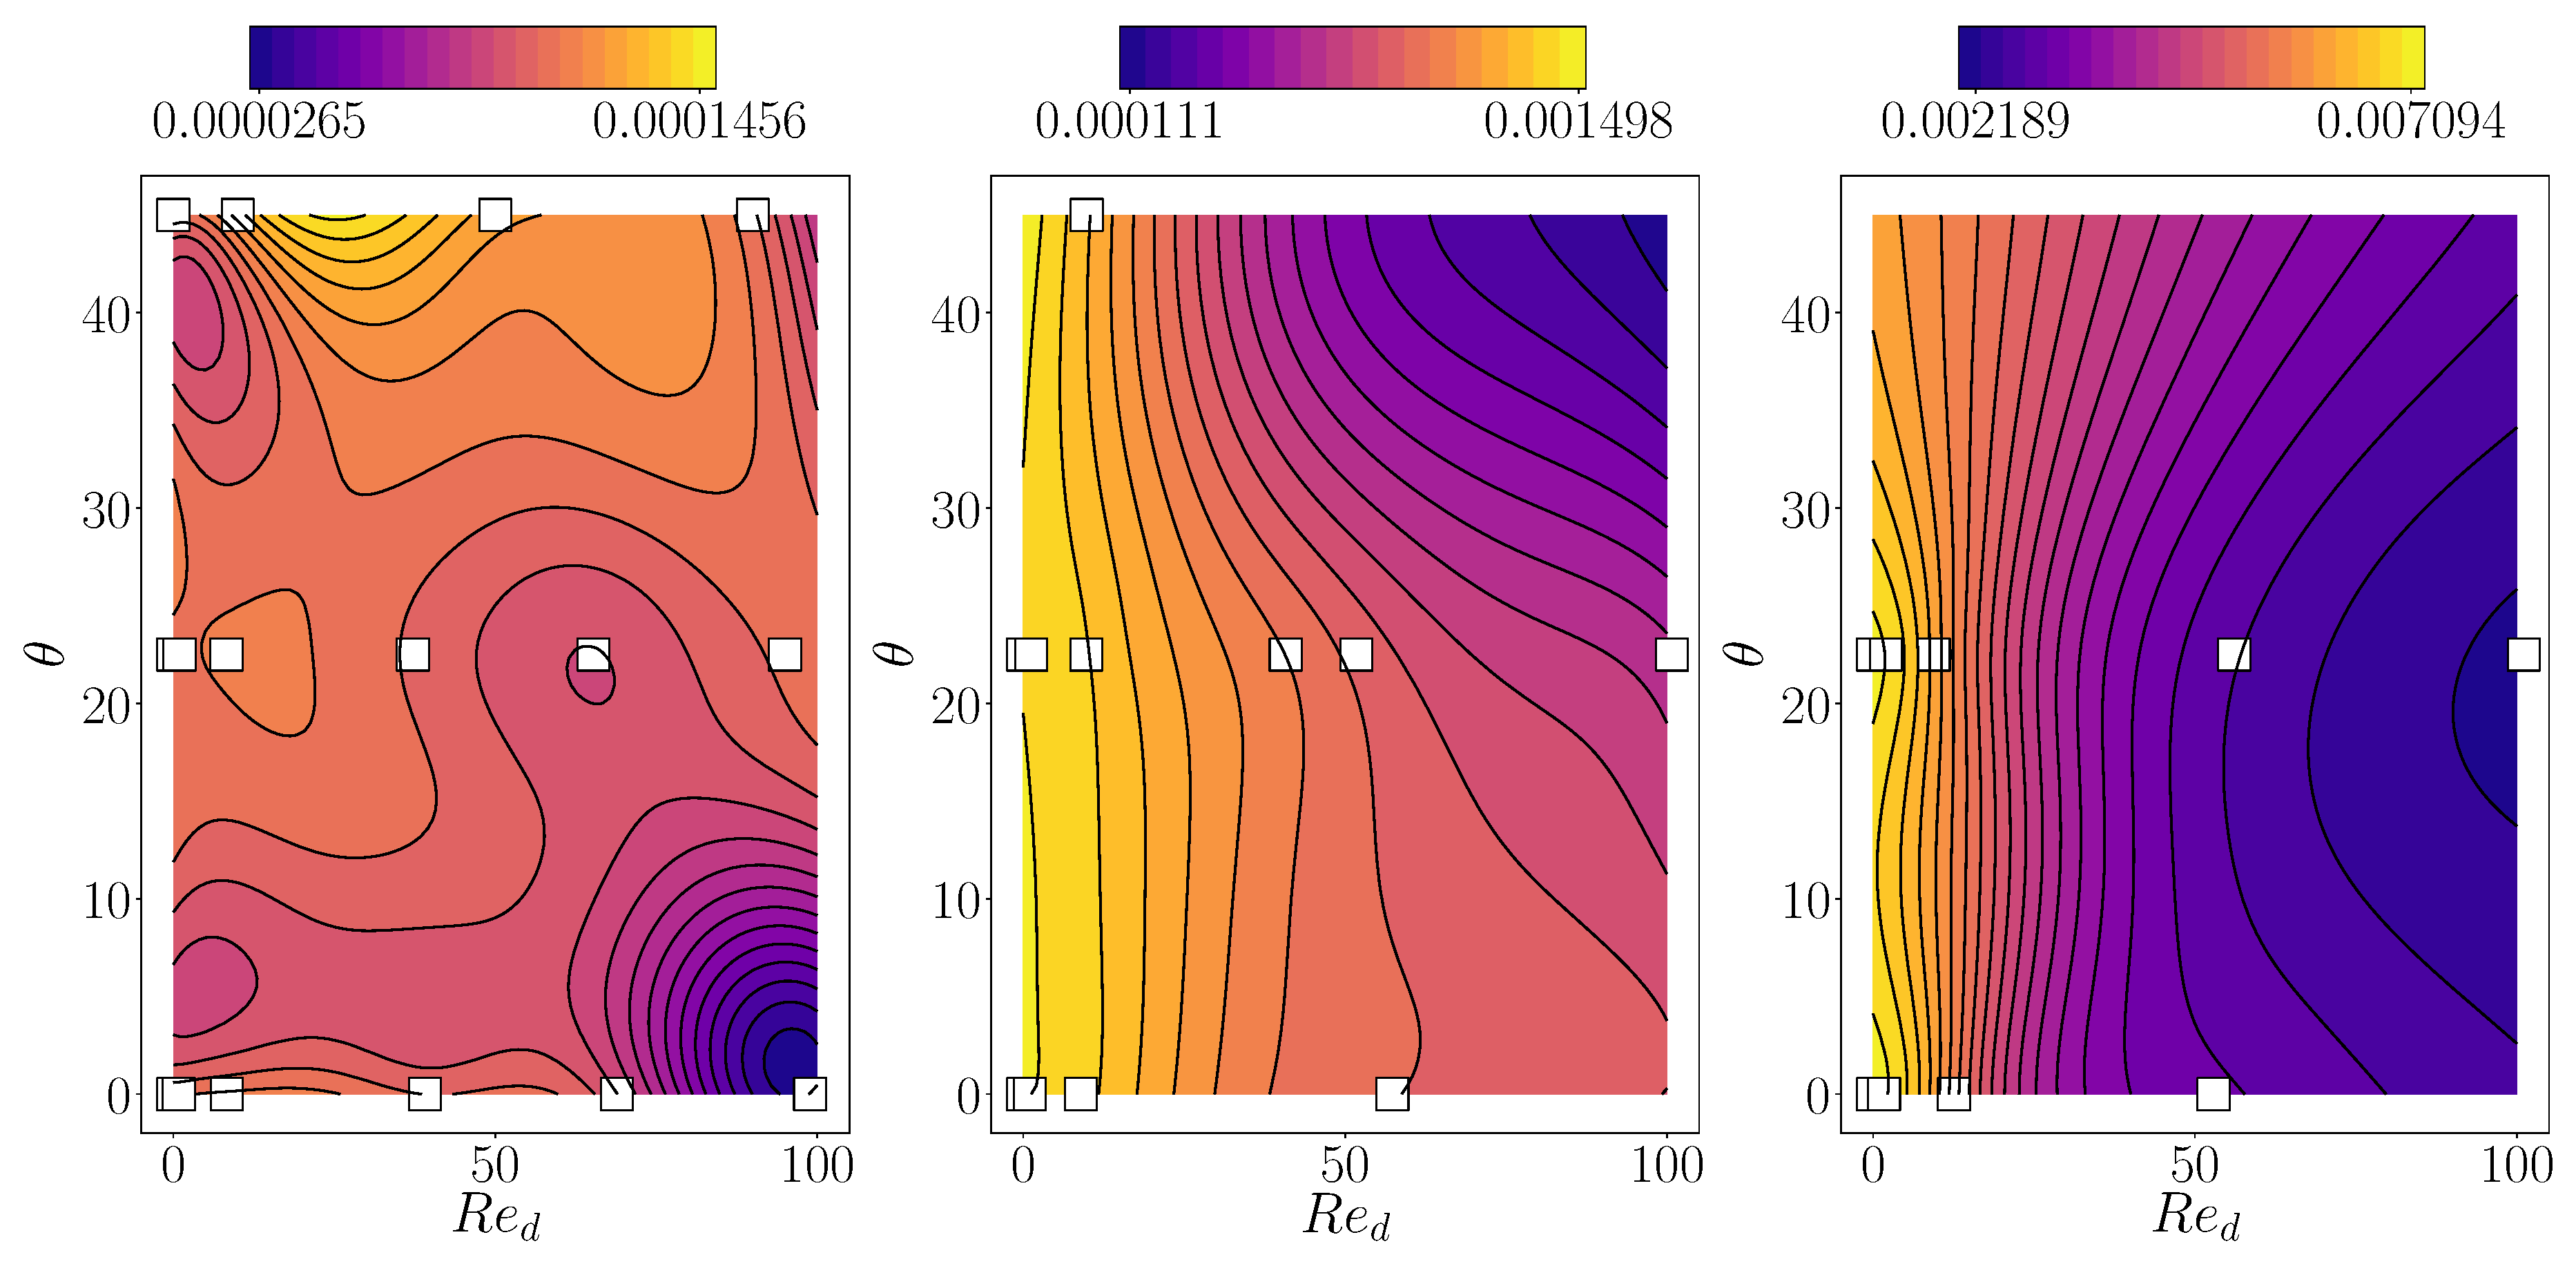
\includegraphics[width=1\linewidth]{chapter_4/figure/krig_mater_th_re}
	\caption{Response surfaces of $H_{11}$ with $\phi=0^{\circ}$ for porosity $\varepsilon=0.4, 0.6, 0.8$, from left to right.}
	\label{fig:th_re}
\end{figure}


In figure \ref{fig:th_re} the angle $\phi$ is fixed to zero, and the isolines display $H_{11}$ as function of the angle $\theta$ and of the 
Reynolds number, $Re_d$, for three  values of porosity.  The white square symbols indicate the  samples used to build the metamodel. The maximum value of 
each surface is always found for $Re_d$ equal to zero and  $H_{11}$  typically decreases with $Re_d$, when the porosity is sufficiently large.
As seen previously, for a porosity approximately greater or equal to 0.6 the variation of the  apparent permeability with the angle $\theta$ 
is weak in this two-dimensional configuration.
For the  lowest porosity studied (left frame)  the permeability has very small values and the isolines display an irregular behaviour; this is a feature
common to all plots relative to the smaller value of $\varepsilon$, signaling that it is probably necessary, in this specific case, to insert additional sample 
points in building the response surfaces. 
%Steep gradients with $Re_d$ are displayed  in the case of horizontal flow ($\theta = 0^{\circ}$).
%The observations made upon inspection of the figure are essentially the same presented in section \ref{sec:5}, and this is comforting, since it leads to
%believe in the  capacity of the metamodel to describe the trend of $H_{11} = f(\theta, Re_d)$.



\begin{figure}[t]
	\centering
	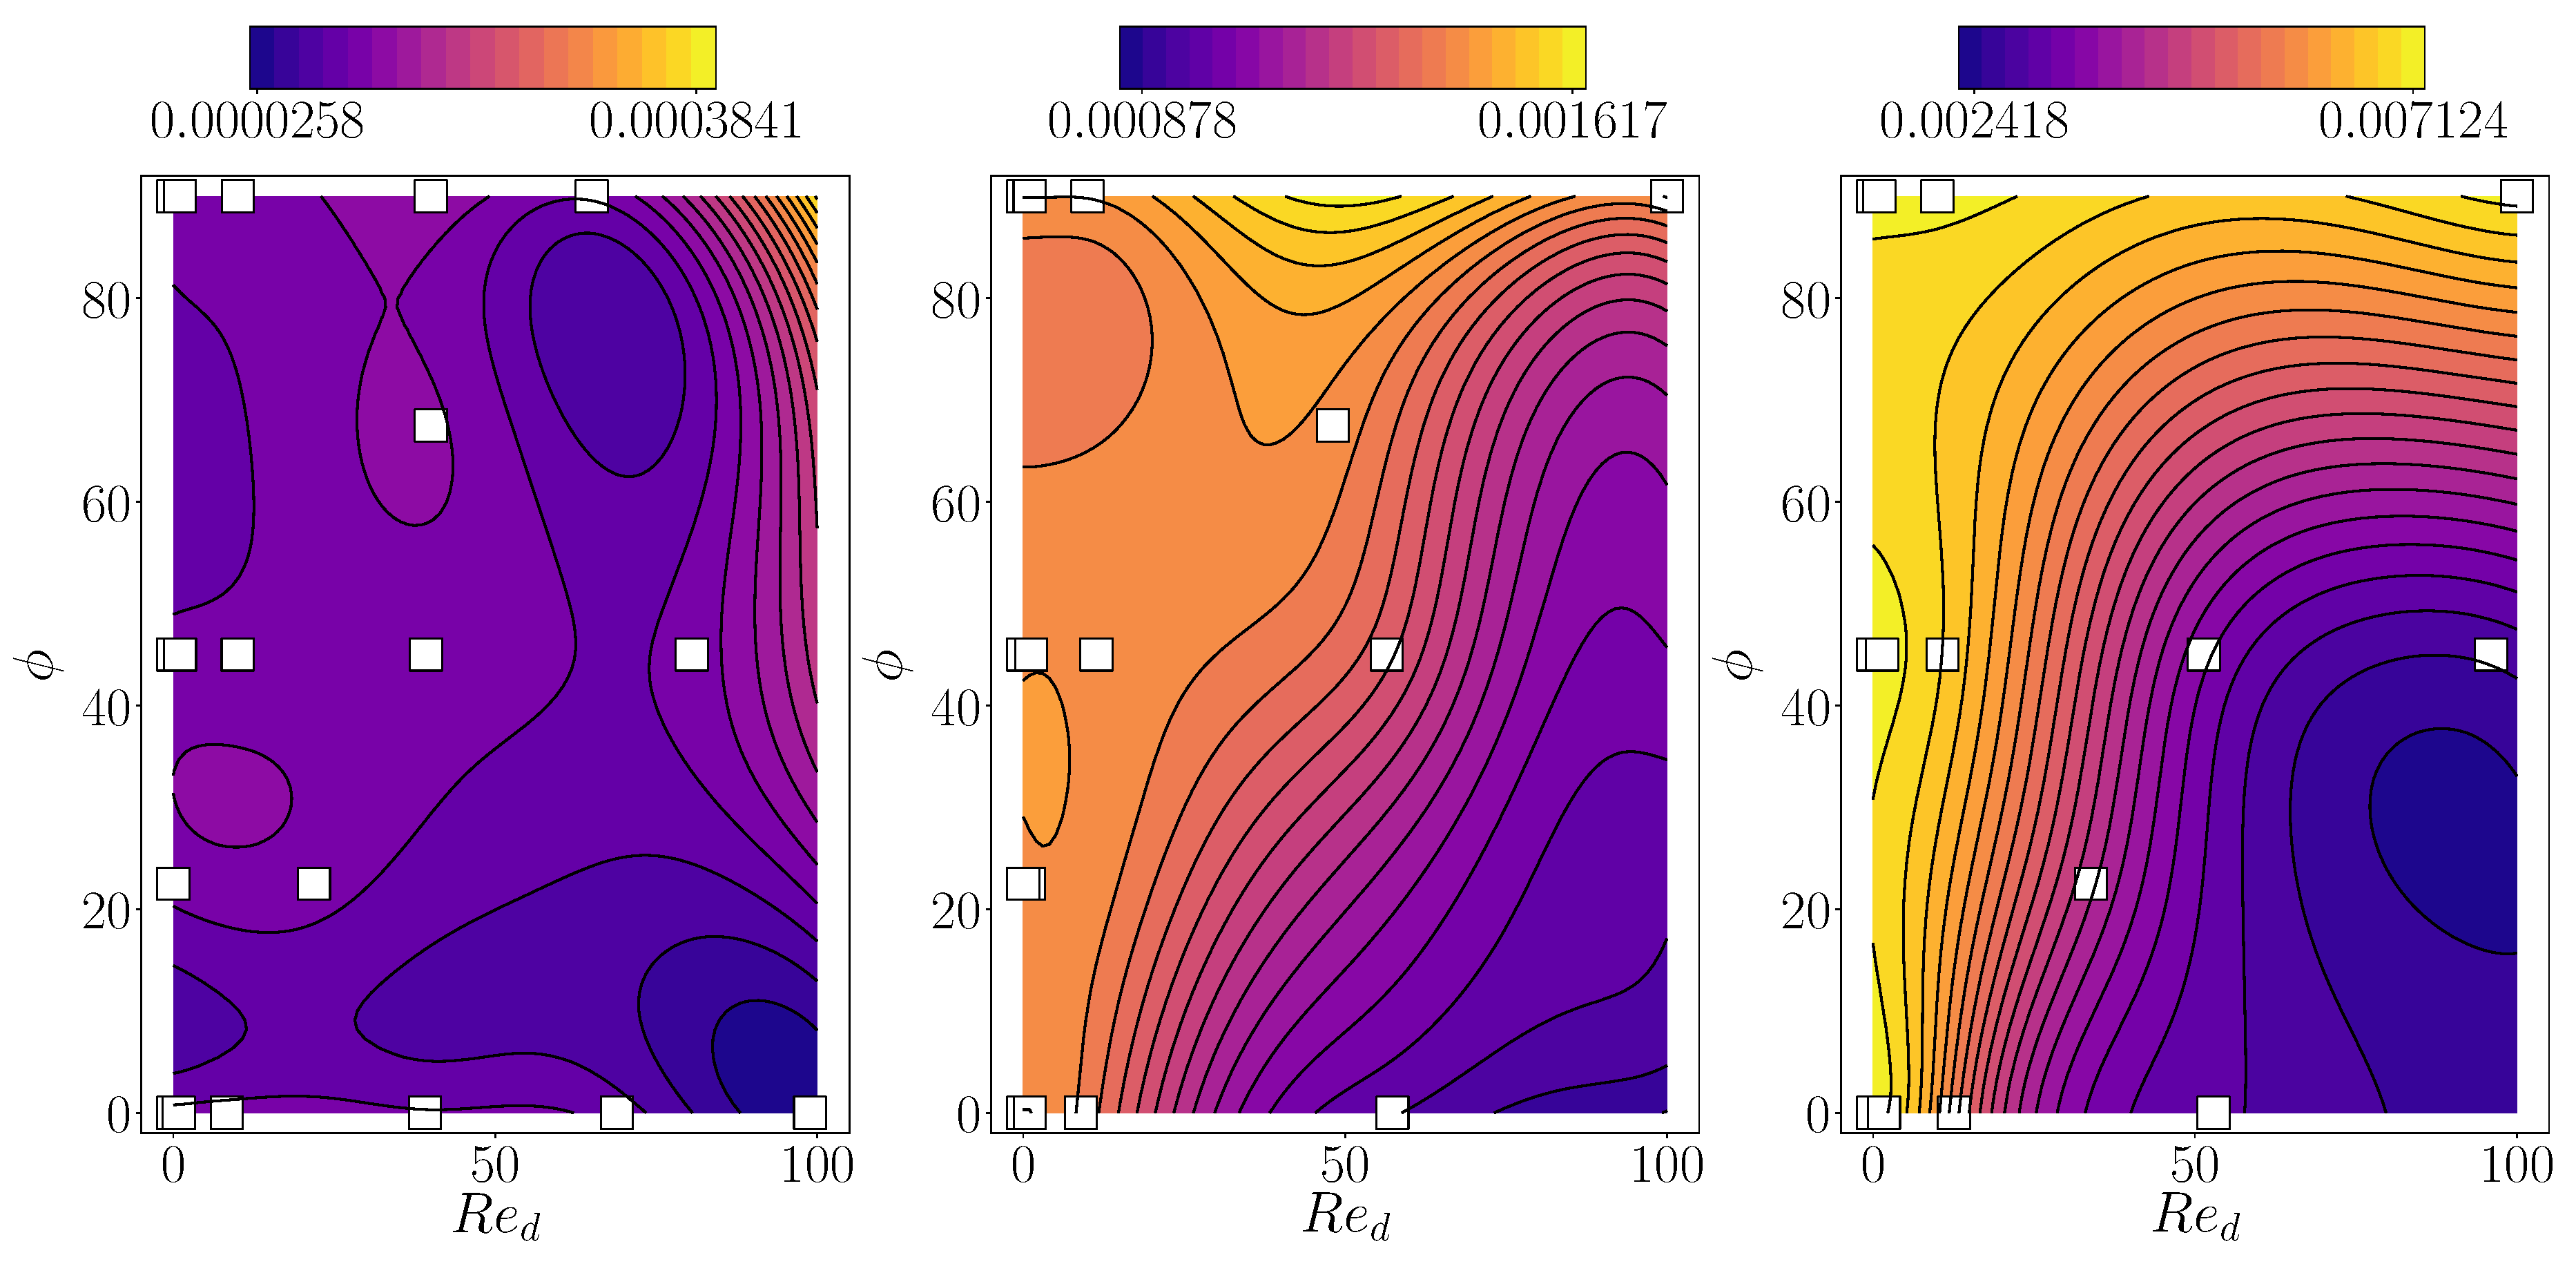
\includegraphics[width=1\linewidth]{chapter_4/figure/krig_mater_ph_re}
	\caption{Response surfaces of $H_{11}$ with $\theta=0^{\circ}$ for porosity $\varepsilon=0.4, 0.6, 0.8$, from left to right.}
	\label{fig:ph_re}
\end{figure}


In  figure \ref{fig:ph_re} the parameter  $\theta$ is set to  $0^{\circ}$ and  the response surface is displayed in the $Re_d - \phi$ plane.
As already indicated, the results confirm that an  increase of  the Reynolds number is generally associated to  a decrease of  the first diagonal component  of the apparent permeability tensor. However, the $H_{11}$ variations with respect to $\phi$ are more pronounced than those found with respect to $\theta$ and are due to a real three-dimensionalization of the flow.
This conclusion remains to be verified in the lower porosity case (left frame) where the variations are very tiny and more irregular.

%For the porosity equals to $0.8$, the surface becomes wavy  around $Re_d = 50$ region. It could be due to the lack of sampled point at this %higher range of Reynolds number. 
%In this region  the surface with porosity equals to $0.6$  shows a more regular variation. Some additional sample could help to explain the %different behaviours.




\begin{figure}[t]
	\centering
	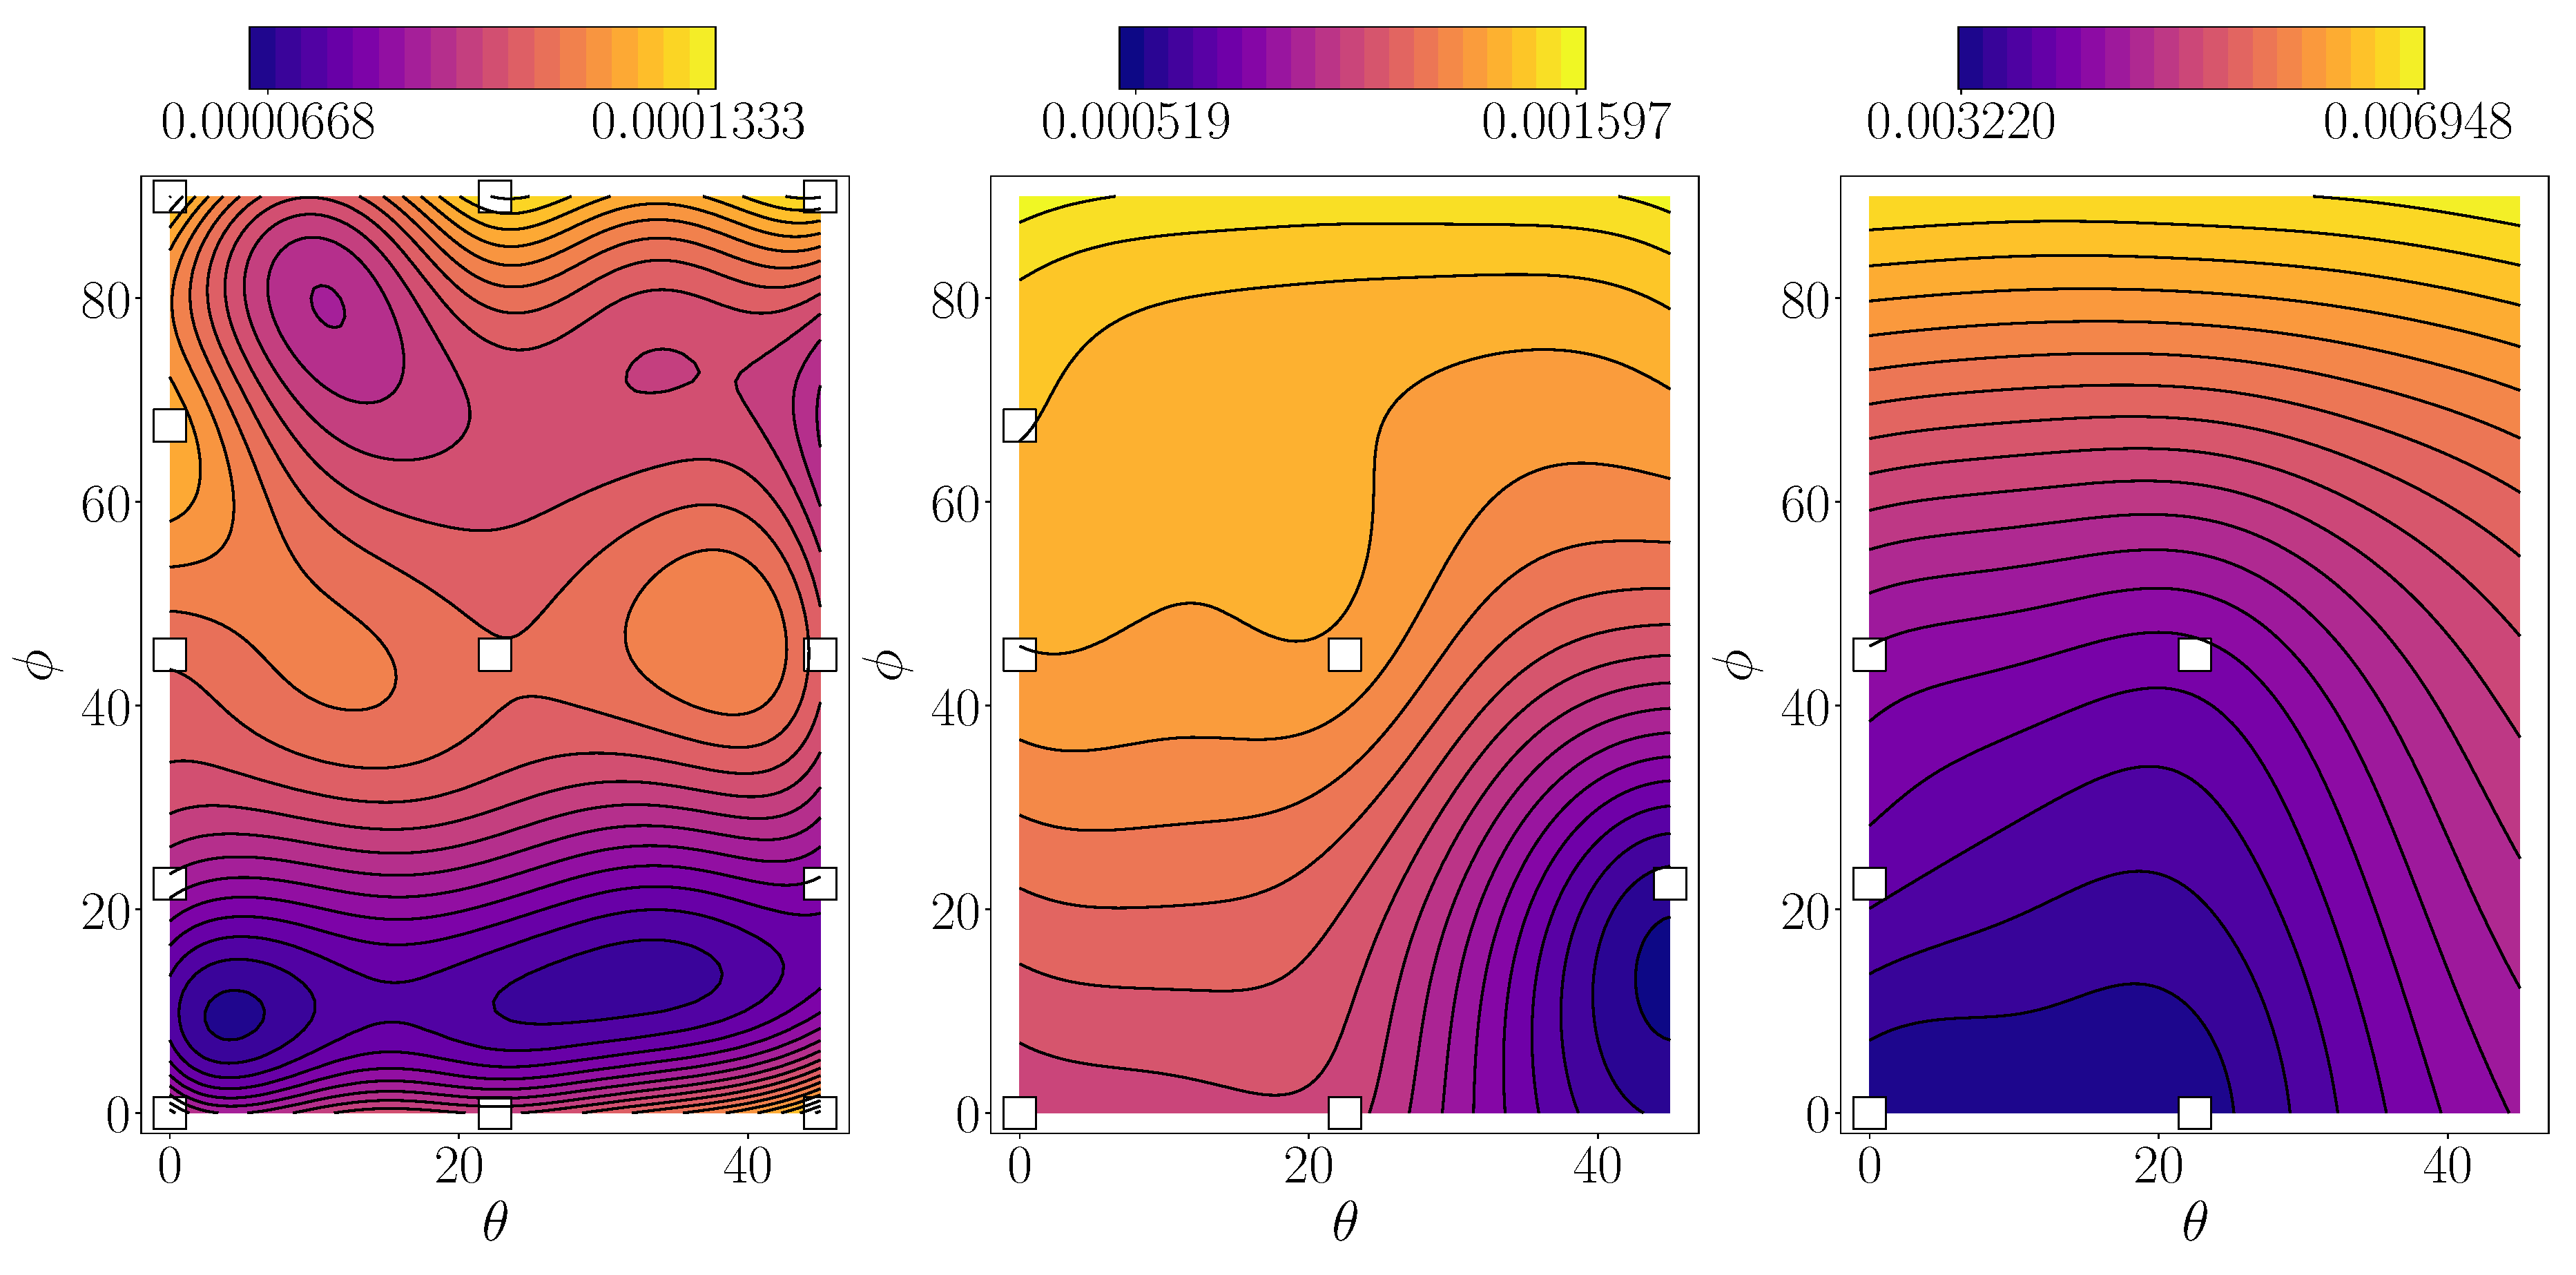
\includegraphics[width=1\linewidth]{chapter_4/figure/krig_mater_th_phi_re40}
	\caption{Response surfaces of $H_{11}$ with $Re=40$ for porosity $\varepsilon=0.4, 0.6, 0.8$, from left to right.}
	\label{fig:th_ph}
\end{figure}


In figure \ref{fig:th_ph} the Reynolds number is set to the inertial range value of $40$ and  the response surface 
is displayed in the $\theta - \phi$ plane. 
For the two highest porosity values, $0.6$ and $0.8$, the results confirm that $H_{11}$ has a much stronger dependence on
$\phi$ than on $\theta$, suggesting that the real test of permeability models must include three-dimensional effects.
As seen earlier, the behaviour of the permeability when the porosity is low (left frame in the figure) is not intuitive, with 
a significant effect of the angle $\phi$ and a minor influence of $\theta$. Again this occurs
from the constraint provided to the flow by the inclusions, and from the occurrence of a large deviation $\gamma$ in these cases.

%shows a strong variability with respect to the angle $\phi$  and a weak one with respect to the angle $\theta$.
%At given Reynolds number the permeability does not depend (too much) of the flow direction in the horizontal plane.
%These conclusions are in agreement with the one observations written in section \ref{sec:4}.

%For the lowest porosity $0.4$ the complex behaviours are retrieved. With respect to the other porosity the variations are inverted : 
%a strong variability with respect to the angle $\theta$ and a weak one with respect to $\phi$ are found.
%As earlier  stated in the previous sections,  with a low porosity the flow direction is deflected towards the fiber axis direction with the %tri-dimensional flow.

%In the range of $\phi < 25^{\circ}$ where the tri-dimensionality remains small  the surface response exhibit a plateau in range $\theta \in %[10^\circ \  30^\circ ]$. The existence
%of this plateau remains unexplained.





The response surface is shown in the $Re_d - \varepsilon$ plane of figure \ref{fig:por} for three sets of $\theta-\phi$ angles. 
Here a significant effect of the porosity with respect to  the Reynolds number is obervable. 
In fact  the surface  gradient is almost aligned with the porosity direction, i.e. a quasi- Reynolds independence is demonstrated  in this plane,
and  the apparent permeability can change by one order of magnitude in the range
of the analysed porosity.

Some relatively small Reynolds number effects are visible at porosity equal to $0.8$, when the wake of the flow has more space to develop in the inertial regime.
In the central figure the flow is aligned with the direction of the fibers and, as expected, it shows practically no dependence with respect to the Reynolds number.


The response surface analysis has confirmed the qualitative trends which had been reached earlier on the basis of a few selected 
flow cases, yielding at the same time much more detailed information on the behaviour of the apparent permeability with the
parameters of the problem. The data base which has been built will be used in future work which will focus, via the VANS approach,
on configurations for which neither the porosity nor the local Reynolds number are constant in space or time.

\begin{figure}[t]
	\centering
	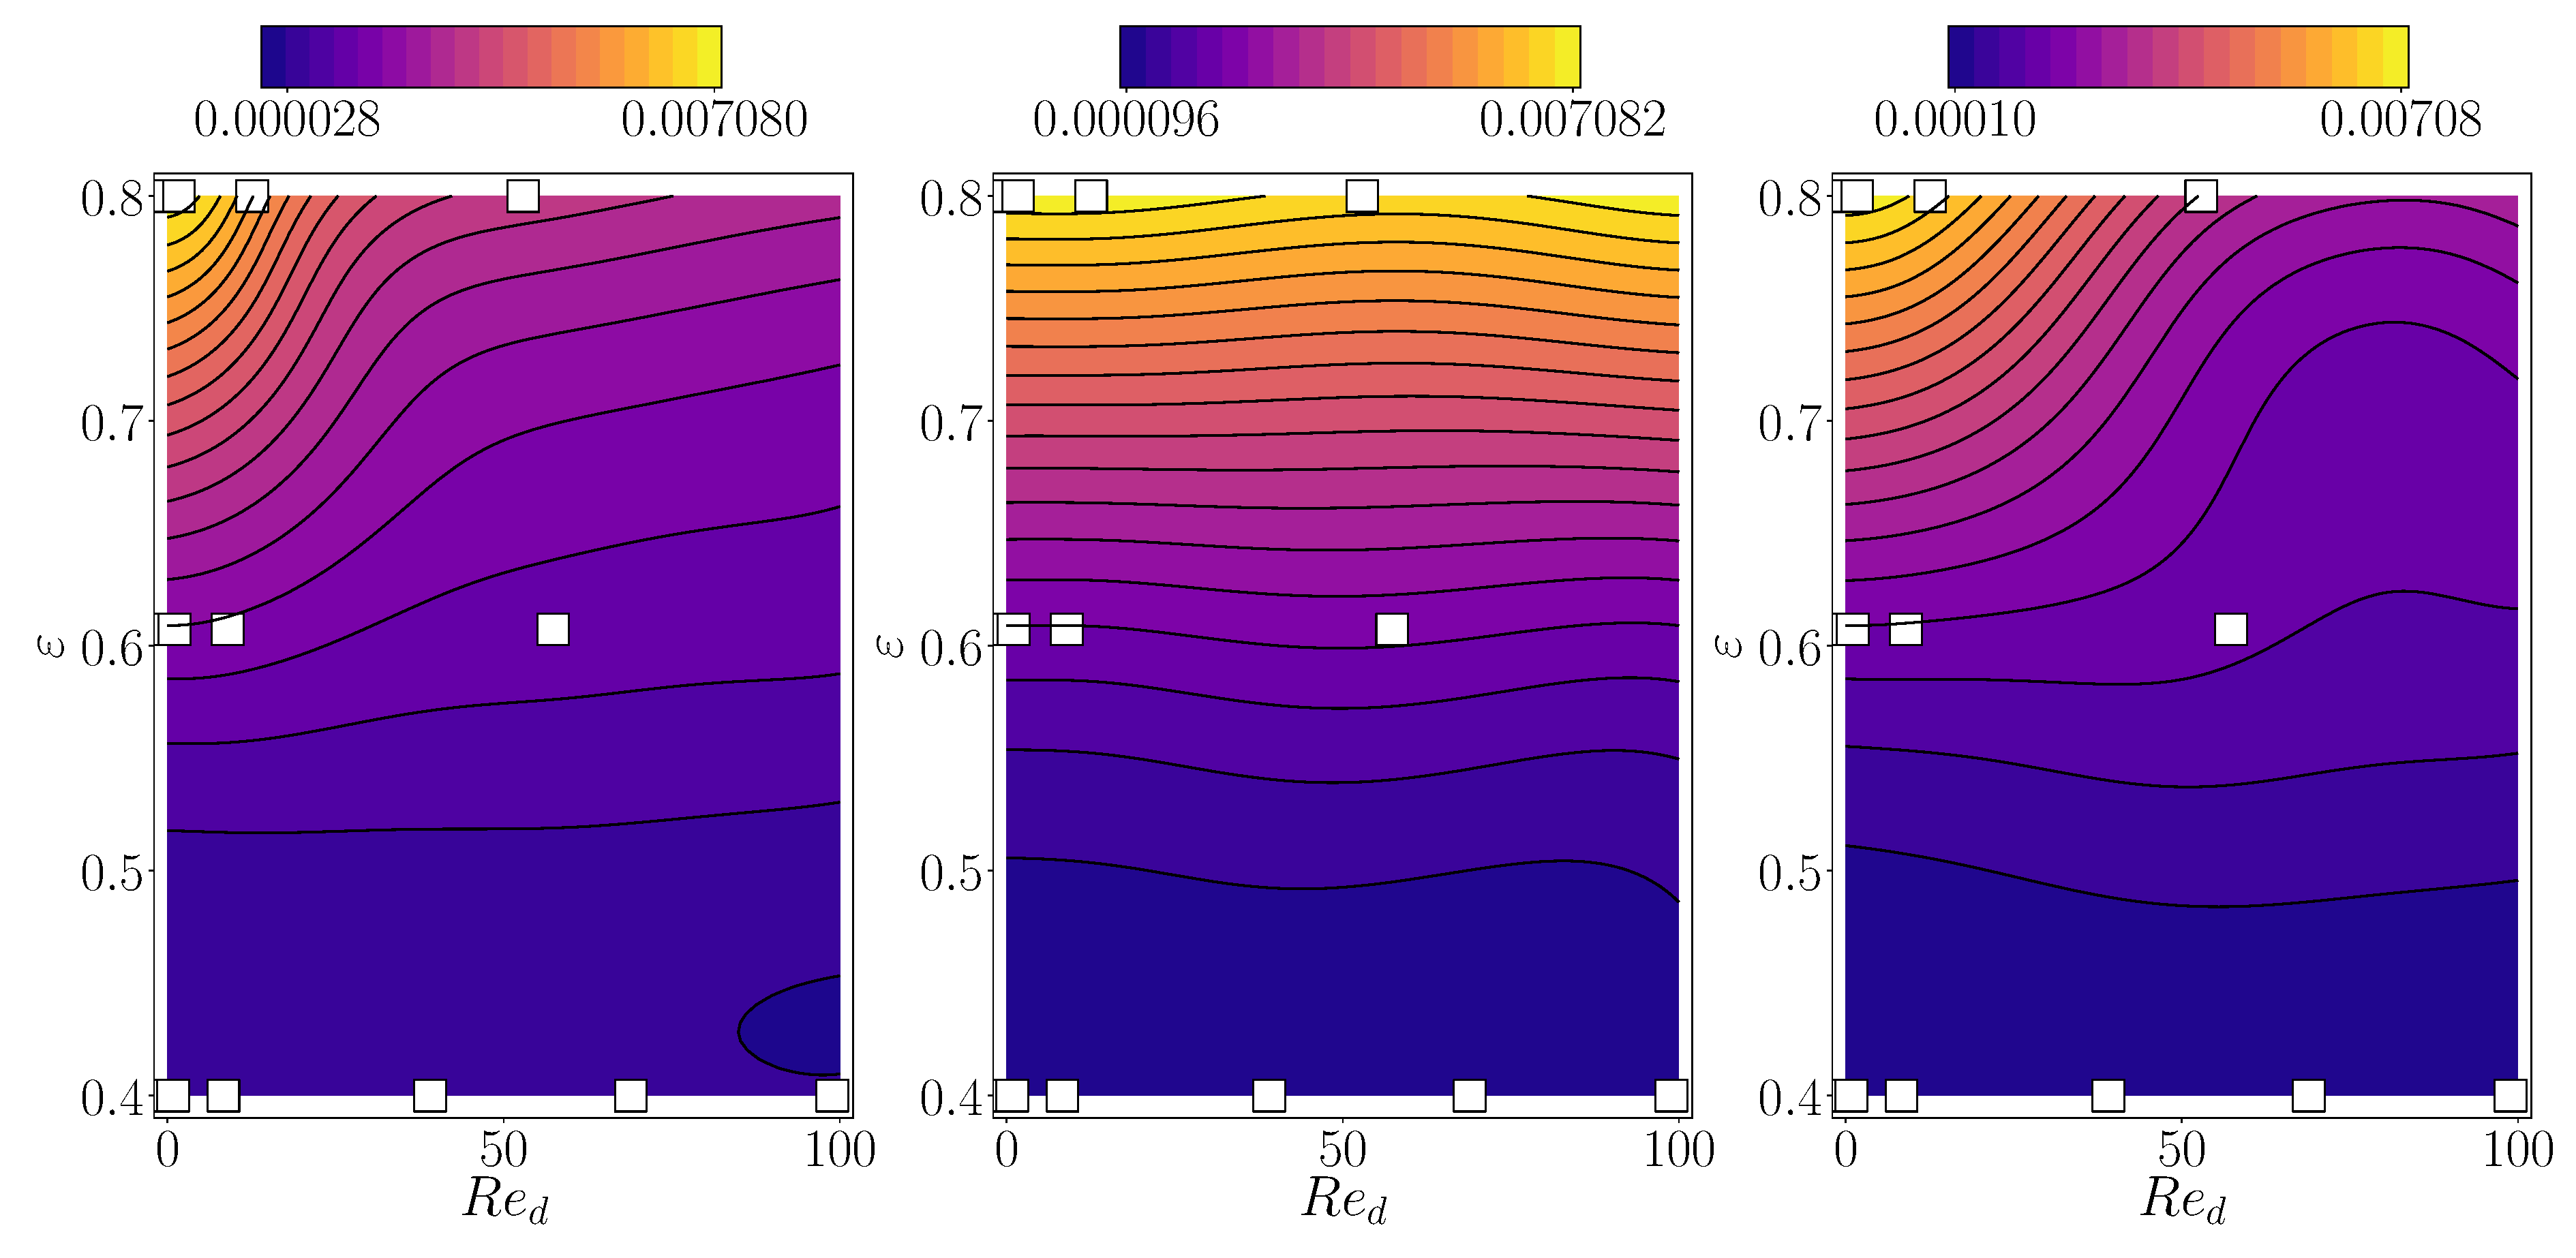
\includegraphics[width=1\linewidth]{chapter_4/figure/krig_mater_eps_re}
	\caption{Response surface of $H_{11}$; in the left frame $\phi= \theta = 0$, in the centre frame $\phi=90^{\circ}$, $ \theta = 0$ and on the right $\phi= 45^{\circ}$, $ \theta = 22.5^{\circ}$.}
	\label{fig:por}
\end{figure}


%%%%%%%%%%%%%%%%%%%%%%%%%%%%%
\section{Concluding remarks}
%%%%%%%%%%%%%%%%%%%%%%%%%%%%%


%%%%%%%%%%%%%%%%%%%%%%%%%%%%%%%%%%%%%%%%%%%%%%%%%%%%%%%%%%%%%%%%%%%%%%%%%%%%%%%%%
%\subsection{Tensors $\mathbf{K}$ and $\mathbf{F}$ by using the VANS system}
%%%%%%%%%%%%%%%%%%%%%%%%%%%%%%%%%%%%%%%%%%%%%%%%%%%%%%%%%%%%%%%%%%%%%%%%%%%%%%%%%

The components of the permeability tensor are essential ingredients for any solution of flow
through anisotropic porous media.  When the flow through the pores resents of significant
acceleration effects, the permeability must be modified (it is then called \emph{apparent}) by the presence
of a second tensor, the Forchheimer tensor $\mathbf{F}$, defined by   
$$
\mathbf{F} =  \mathbf{K} \mathbf{H}^{-1} - \mathbf{I}.
$$
The permeability, $\mathbf{K}$, and the apparent permeability, $\mathbf{H}$, can be formally deduced by two closure problems which have
been briefly recalled in section \ref{sec:2ch4}.  The real obstacle to the solution of the problem for $\mathbf{H}$ is the need
to know the microscopic velocity fields through the pores. We have solved for such fields 
in a unit cell (the REV), varying the forcing amplitude and direction, treating over one
hundred different cases of flows through arrangements of parallel fibers. From this, we have
thus been able to solve the linear system \eqref{eq:linear_k} for all the unknown elements of the 
intermediate tensor  
$\mathbf{M}$, from which, through averaging, we have computed the apparent permeability.  Such a tensor
is  indispensable to evaluate accurately the drag force caused by the presence of the fibers, for a macroscopic solution of the flow on the
basis of equations \cite{whitaker2013method} when inertial effects are present.

It has been found that the apparent permeability tensor is strongly diagonally dominant for whatever
forcing direction and porosity,  provided the local Reynolds number remains below a value 
approximately equal to 100; this results -- which is a direct
consequence of the transverse isotropy of the material which has been considered here -- 
can be used to compute $\mathbf{H}$ rapidly, approximating it as a diagonal tensor.

Finally, a metamodel has been used to produce results so as to cover the whole space of parameters,
and this has allowed the construction of a complete data base.  This data base is now being used in simulations of poroelastic media based on the VANS approach. 
